%                                                  Last change: 02/10/2016
\documentclass[review]{elsarticle}

\usepackage{lineno,hyperref}
\usepackage{array}

\modulolinenumbers[5]

\journal{Medical Engineering \& Physics}

%% `Elsevier LaTeX' style
\bibliographystyle{elsarticle-num}
%%%%%%%%%%%%%%%%%%%%%%%

%\documentclass[twocolumn]{autart}    % Enable this line to obtain a two-column
                                     % document whose style resembles the
                                     % printed Automatica style.

%\documentclass[final,4p,times,twocolumn,authoryear]{elsarticle}



%\usepackage[T1]{fontenc}
%\usepackage[dvips]{graphicx}
%\usepackage[dvips]{color}
%\usepackage{amsfonts}
%\usepackage{amsmath}
%\usepackage{multicol,anysize}%,amsthm}
%\usepackage{latexsym}
%\usepackage{amssymb}
% %%%%%%%%%%%%%%%%%%%%%%%%%%%%%%%%%%%%%%%%%%%%%%%%%%%%%
\usepackage[latin1]{inputenc}
\usepackage{epstopdf}
% \usepackage[T1]{fontenc}                                                        
% % by Nerito
% \usepackage{latexsym}
\usepackage{xcolor}
% \usepackage{graphicx}
% \usepackage[scanall]{psfrag}
% % FONTES MATEMATICAS
\usepackage{amsmath}     % Simbolos matematicos ams
\usepackage{amssymb}     % Simbolos matematicos adicionais do AmS
% \usepackage{amsfonts}    % Pacotes Tipicos c/ fontes matematicas
% \usepackage{amstext}
% \usepackage{latexsym}    % Simbolos matematicos adicionais
% \usepackage{mathrsfs}
% \usepackage{bm}          %makes bold greek ${\bm \alpha}$
% \usepackage{amsopn}
% \usepackage{hyperref}
% \usepackage{url}
% %%%%%%%%%%%%%%%%%%%%%%%%%%%%%%%%%%%%%%%%%%%
%
% \hyphenation{}
% %\theoremstyle{plain}
% \newtheorem{property}{Property}
% \newtheorem{proposition}{Proposition}
% \newtheorem{definition}{Definition}
\newtheorem{lemma}{Lemma}
% \newtheorem{corollary}{Corollary}
\newtheorem{theorem}{Theorem}
\newtheorem{remark}{Remark}
% \newtheorem{example}{Example}
% 
% \usepackage{amssymb}
% \usepackage{anysize}
% \marginsize{1.5cm}{1cm}{3cm}{0.7cm} %lrtb
% %
% % my commands
% \newcommand\norm[1]{\ensuremath{\lVert#1\rVert}}
% \newcommand\abs[1]{\ensuremath{\lvert#1\rvert}}
% \newcommand{\sign}{\operatorname{sign}}
\newcommand{\sgn}{\operatorname{sgn}}
\newcommand{\proof}{\textbf{Proof:~}}
% %\newcommand{\endproof}{$\box$}
% \def\endproof{$\Box$}
% %\newcommand{\meuendereco}{ COPPE/UFRJ --- Department of Electrical Engineering ,
% % P.O. Box 68504, 21945--970 --- Rio de Janeiro --- BRAZIL }



\begin{document}

\begin{frontmatter}

\title{Time-scaling based Sliding Mode Control for Neuromuscular Electrical Stimulation under\\ Uncertain Relative Degrees }


\author[mymainaddress]{Tiago Roux Oliveira\corref{mycorrespondingauthor}}
\cortext[mycorrespondingauthor]{Corresponding author}
\ead{tiagoroux@uerj.br}
\author[mysecondaryaddress]{Luiz Renn\'{o} Costa}
\author[mysecondaryaddress]{Joao Marcos Yamasaki Catunda}
\author[mysecondaryaddress]{Alexandre Visintainer Pino}
\author[mymainaddress]{William Barbosa}
\author[mysecondaryaddress]{Marcio Nogueira de Souza}


\address[mymainaddress]{Dept. of Electronics and Telecommunications, State University of Rio de Janeiro (UERJ), Rio de Janeiro, RJ 20550-900, Brazil.}
\address[mysecondaryaddress]{Biomedical Engineering Program, Federal University of Rio de Janeiro (COPPE/UFRJ), Rio de Janeiro, RJ 21945-970,
P.O. Box 68510, Brazil.}



\begin{abstract}                          % Abstract of not more than 200 words.
%%%%%%%%%%%%%%%%%%%%%%%%%%%%%%%%%%%%%%%%%%%%%%%%%%%%%%%%%%%%%%%%%%%%%%%%%%%%%%%%
\begin{small}
This paper addresses the application of the sliding mode approach to control the arm movements by artificial recruitment of muscles
\textcolor{black}{using} Neuromuscular Electrical Stimulation (NMES). Such a technique allows the activation of motor nerves using surface electrodes. 
The \textcolor{black}{goal} of the proposed control system \textcolor{black}{is} to move the upper limb of \textcolor{black}{subjects} through electrical stimulation to achieve a desired elbow angular displacement. Since the human neuro-motor system has individual characteristics, being time-varying, nonlinear and subject to uncertainties, the use of advanced robust control schemes may represent a better solution than classical Proportional-Integral (PI) controllers \textcolor{black}{and model-based approaches, being simpler than more sophisticated strategies using fuzzy logic or neural networks}, usually applied in this control problem. The objective is the introduction of a new time-scaling base sliding mode control strategy for NMES and its experimental evaluation. The main qualitative \textcolor{black}{advantages} of the proposed controller via time-scaling procedure \textcolor{black}{are} its independence of the knowledge of the plant relative degree and the design/tuning simplicity. \textcolor{black}{The developed sliding mode strategy allows for chattering alleviation due to the impact of the integrator in smoothing the control signal. In addition, no differentiator is applied to construct the \textcolor{black}{sliding surface.}} The stability analysis of the closed-loop system is also carried out by using singular perturbation methods. \textcolor{black}{Experimental results are conducted with healthy volunteers as well as stroke patients.}  \textcolor{black}{Quantitative results show a reduction of
$45\%$ in terms of root mean square (RMS) error (from $5.9^{o}$ to $3.3^{o}$) in comparison with PI control scheme, which is similar to that obtained in the literature.}
\end{small}
%%%%%%%%%%%%%%%%%%%%%%%%%%%%%%%%%%%%%%%%%%%%%%%%%%%%%%%%%%%%%%%%%%%%%%%%%%%%%%%%%%%
\end{abstract}


\begin{keyword}                           
\textcolor{black}{stroke patients}; uncertain systems; functional electrical stimulation; sliding mode control; output feedback; trajectory tracking; singular perturbation.
\end{keyword}


\end{frontmatter}

\linenumbers

%%%%%%%%%%%%%%%%%%%%%%%%%%%%%%%%%%%%%%%%%%%%%%%%%%%%%%%%%%%%%%%%%%%%%%%%%
\section{Introduction}

\textcolor{black}{Electrotherapy} has been used for the treatment of paralysis, contractions and other nervous diseases \cite{D:2008}. With the advances in electronics and informatics, medical equipments for such purposes  became specialized and \textcolor{black}{portable}, opening a new range of options to this type of treatment, as Neuromuscular Electrical Stimulation (NMES) \cite{M:2010}. 

The NMES technique is based on electrically  generating muscle contractions through activation of intramuscular nerve branches \cite{SC:2007}. 
Although the use of NMES \textcolor{black}{has effects} on motor recovery of stroke patients mostly evident on upper limbs, it is also very commonly used for lower extremities, \textcolor{black}{such as the treatment of drop foot \cite{Seel2016_CEP}.} 
In addition, it helps the recovery of muscle strength in upper and lower limbs \cite{R:2003}, \cite{VWPWHRK:2014}.
NMES  \textcolor{black}{has also been} explored to enable spinal cord injured individuals to make grasping, standing and another functional movements, being \textcolor{black}{a useful} tool \textcolor{black}{in the rehabilitation process of paralysis and stroke patients \cite{LP:2008}, \cite{S:82}, \cite{H:2008}, \cite{JWK:2004}, \cite{ZPWA:2011}, \cite{VHA:2012}, \cite{DTLZ:1999}, \cite{FHBC:2009}, \cite{PFSB:2005},
\cite{BPYSSP:2015}, \cite{BRD:2009}.}




In order to improve the movements produced or aided by NMES, there is a need for control algorithms that can handle patients 
variability, external disturbances and uncertainties \cite{BFF:2015}, \cite{H:2008}. 
For precise closed-loop feedback control of NMES, a mathematical description of electrically stimulated
muscle is vital. However, identification of such a model is widely seen as impractical in a clinical setting due to time
constraints and rapidly changing dynamics (due to fatigue, spasticity, and \textcolor{black}{shifting} physiological and environmental
factors such as skin impedance, temperature, and electrode placement). Thus, there are many mathematical models of the human neuro-motor system which are in general time-varying, nonlinear and different for each  individual \cite{NH:94}, \cite{DKFD:2016}, \cite{VHA:2012}, \cite{P:2002}, \cite{L:12}, \cite{SNPHFFR:2005}, \cite{LMFR:2010},
\cite{XCR:2014}, \cite{FHBC:2008}. 


In this context, models with uncertain relative degrees are often common and represent a challenging task \cite{L:2012}. Motivated by this issue, the concept of practical relative degree was introduced in another biomedical control application \cite{HFLSLMA:2013} to facilitate the design of a differentiator based quasi-continuous higher-order sliding mode control for blood glucose regulation. \textcolor{black}{However, the use of differentiators increases the sensitivity of the closed-loop system with respect to measurement noise, sampling discretization and time delays \cite{L:2000}. As a rule of thumb: the higher relative degree, the higher sensitivity \cite{Lev:03}, \cite{OPH:2013}.}  


\textcolor{black}{A known weak point of most control approaches for NMES is the 
\textcolor{black}{need for a well defined, constant, and known system relative degree}  
\cite{JWK:2004}, \cite{SGD:2011}, \cite{KMQKY:2014}, \cite{MPFG:2012}, \cite{DTLZ:1999}, \cite{FHBC:2009}, \cite{PFSB:2005}, \cite{XCR:2014}, \cite{FE:2014}, \cite{NE:2012}.} On the other hand, any small perturbation or model inaccuracy can lead to the increase/decrease of the relative degree, or even to its disappearance \cite{L:2012}. In addition, a lengthy identification procedure would be required at the beginning of each NMES treatment session, and any unpredictable rapid variation in the system could degrade the performance of the treatment \cite{BFF:2015}. Thus, the use of advanced control techniques robust to model order variations and parametric uncertainties is welcome and may be more appropriate to stabilize biological or biomedical processes. 

\textcolor{black}{In the output-feedback control design described in \cite{L:2000} using differentiators, the relative degree of the dynamic system must be known. Since the relative degree of the controlled system is considered unknown for the user in our approach, it would impose an additional difficulty in the observers/differentiators implementation due to \textcolor{black}{the lack of knowledge regarding the exact order} of the neuromuscular model. This makes our strategy innovative, since less information of the model is required when compared with the existing literature.}

 




This paper proposes a robust sliding mode controller free of differentiators and \textcolor{black}{implements} it to a custom NMES device. The designed scheme aims to move the upper limbs through electrical stimulation to achieve predetermined \textcolor{black}{angle trajectory reference.} 
\textcolor{black}{Despite that,} the control and movement of other joints could be envisaged following the same idea. It is expected \textcolor{black}{to show} experimentally the efficacy of the proposed controller in terms of root mean square (RMS) error,
\textcolor{black}{when compared} to classical approaches such as \textcolor{black}{a} Proportional-Integral (PI) compensator.
\textcolor{black}{We have considered tests with healthy volunteers and stroke patients in order to support the final objective of our control application for motor rehabilitation of stroke patients.}

The convergence of the closed-loop system to a small neighborhood close to the desired reference signal is demonstrated by using
singular perturbations methods. The main theoretical contribution is the development of a time-scaling technique which reduces the order of the dynamical system, and therefore, allows the analysis and design of the sliding mode controller without the exact knowledge
\textcolor{black}{regarding} the relative degree of the plant model. The experimental results illustrate the performance of proposed control algorithm for NMES.

 

\section{\textcolor{black}{Prototype and Experimental Setup}}
\label{protocol}

\textcolor{black}{
Healthy volunteers \textcolor{black}{as well as stroke patients} were recruited for the experiments. 
The subjects \textcolor{black}{were seated with both arms rested on the table, strapped alongside the aluminum bar system (Figure~\ref{fig4}).}
%
%\newpage
\begin{figure}[!htb]
\begin{center}
%\hspace{0.0cm}
\includegraphics[width=0.7\textwidth]{fig4_new.pdf}
%\includegraphics[width=8.5cm]{Figures/fig4.eps}
\caption{\textcolor{black}{Volunteer positioned for the NMES experiment. The controlled joint angle is denoted by $y$.}}
\label{fig4}
\end{center}
\end{figure}
%
%
A mechanical apparatus was built in order to keep the movement restricted to an elbow flexion and extension, and avoid shoulder rotations. In Figure~\ref{fig4_new}, we present the mechanical parts of the apparatus developed for our NMES experiments. The built NMES test bed may be used for contra-lateral motion (moving one voluntarily arm and other electrically stimulated) or movements of a single limb with trajectory reference provided by a computer. 
%
\begin{figure}[!htb]
\begin{center}
%\hspace{0.0cm}
\includegraphics[width=1\textwidth]{aparatops.pdf}
%\includegraphics[width=8.5cm]{Figures/fig4.eps}
\caption{Mechanical apparatus \textcolor{black}{used to limit NMES experimental tests to a single degree of freedom.} The point $A$ in the image indicates a goniometer (simple potentiometer) linked to a steel axis $B$ allowing angular displacement readings. Letter $C$ shows that the wrist has an attachment with linear freedom of movement along the aluminum square rod, while $D$ points out that there is an adjustment for the lateral distance of the elbow.}
\label{fig4_new}
\end{center}
\end{figure}
%
}

 
\textcolor{black}{Electrodes for electrical stimulation must be placed at the motor points of biceps brachii muscle (BB) and triceps brachii muscle (TB). In order to find the motor points,
a small pen electrode of 1 $\text{cm}^2$ area was moved over the skin using 1 Hz pulses at 400 $\mu$s pulse-width of increasing current amplitudes looking for the point with the biggest twitch \textcolor{black}{applying} the smallest current. Then, two self-adhesive \textcolor{black}{square shaped electrodes} with 5 cm of side were used, one on the motor point and the
other 2 cm distal (the electrodes can be seen on the biceps muscle of the volunteer in Figure\ref{fig4}). }


The NMES device has two output channels, \textcolor{black}{which allow} simultaneous stimulation of the BB and TB. The use of two independent channels \textcolor{black}{enables} the controller \textcolor{black}{to act upon} the elbow joint at flexion and extension movements, while the elbow angle (Figure~\ref{fig4}) is measured by a goniometer. \textcolor{black}{Pulse width, frequency, and amplitude (current) could be programmed by computer. The stimulator is controlled via universal serial bus (USB) port and the user interface has been developed at \textcolor{black}{LabVIEW 8.5 (National Instruments, USA)}, which also reads data from a NI USB-6009 14 bit analog-to-digital converter
(National Instruments, USA). A dedicated microcontroller PIC32MX795F512L (Microchip, USA) is used to control the NMES device.}



\textcolor{black}{The stimulation intensity is a function of the total charge transferred to the muscle, which depends on the pulse amplitude, duration, and frequency. 
A typical stimulation pulse used for NMES is a biphasic square-wave pulse train. 
In our tests, the pulse train is symmetric in amplitude (positive or negative), with $50$ Hz \cite{LP:2008} and 
a pulse duration of 400$\mu$s ($200 \mu$s for the positive part and $200 \mu$s for the negative part). }
The controller modulates the current at each pulse. A biphasic waveform is used because it induces charge transfer into the tissue and then immediately induces it out. This pattern of charge 
transfer prevents galvanic processes that can cause tissue damage. Notice that the amount of charge transferred into the tissue is the same as the charge transferred out of the tissue \cite{LP:2008}. 


\textcolor{black}{
A current limiter was implemented saturating the control signal, which has been used to avoid discomfort for the subject during the experiments.} The current limit value can be identified stimulating each BB and TB muscles for short periods of time using progressively higher currents until the volunteer reports the stimulation was uncomfortable. The maximum value of current tolerated is patient dependent and must be individually assessed for each subject. 



\section{\textcolor{black}{Empirical Model for the Open-Loop System}}
\label{empirical}


\textcolor{black}{This section illustrates the nonlinear nature of the open-loop system
\textcolor{black}{through the violation of the} 
\textit{superposition principle} as well as the time-varying behavior of the neuromusculoskeletal system.}



\textcolor{black}{In Figures~\ref{fig5} and \ref{fig50}, the open-loop experimental tests were performed with the same patient. In the former
were obtained different qualitative responses (overshoot and settling time) for %a given reference target (elbow angle of $45^o$) and
input current signals with different magnitudes. For instance, \textcolor{black}{the dead-zone phenomenon \cite{SNPHFFR:2005}} is clearly verified in our experiments: the patient does not respond to any value of current stimulation. The muscles just respond after the current value has crossed some threshold (e.g., 36 mA as in Figure~\ref{fig5}). In a few words, there is a minimal value of electrical stimulation for which the muscle starts up the movement. On the other hand, the time-varying behavior of the neuromusculoskeletal plant is shown in Figure~\ref{fig50}, for the same input \textcolor{black}{applied at two different time instants.}}




\textcolor{black}{In spite of this, it is easy to check the neuromusculoskeletal model in \textbf{open loop} is input-to-state stable (ISS) \cite[p. 175]{K:2002} in the sense that for any bounded input the state variables (and output signal) are bounded too, even in the presence of the delays. This is a reasonable assumption that can be supported by the physical nature of the neuromusculoskeletal model of the plant and the observed open-loop responses. Note that, we do not need to test every possible bounded input signal to realize or conclude that the measured joint angle (output signal) or the internal states of the mathematical representation will never explode neither grow unboundedly.}

%
\begin{figure}[!htb]
%\hspace{-0.8cm}
\begin{center}
%\includegraphics[width=.44\textwidth]{Figures/fig5.eps}
%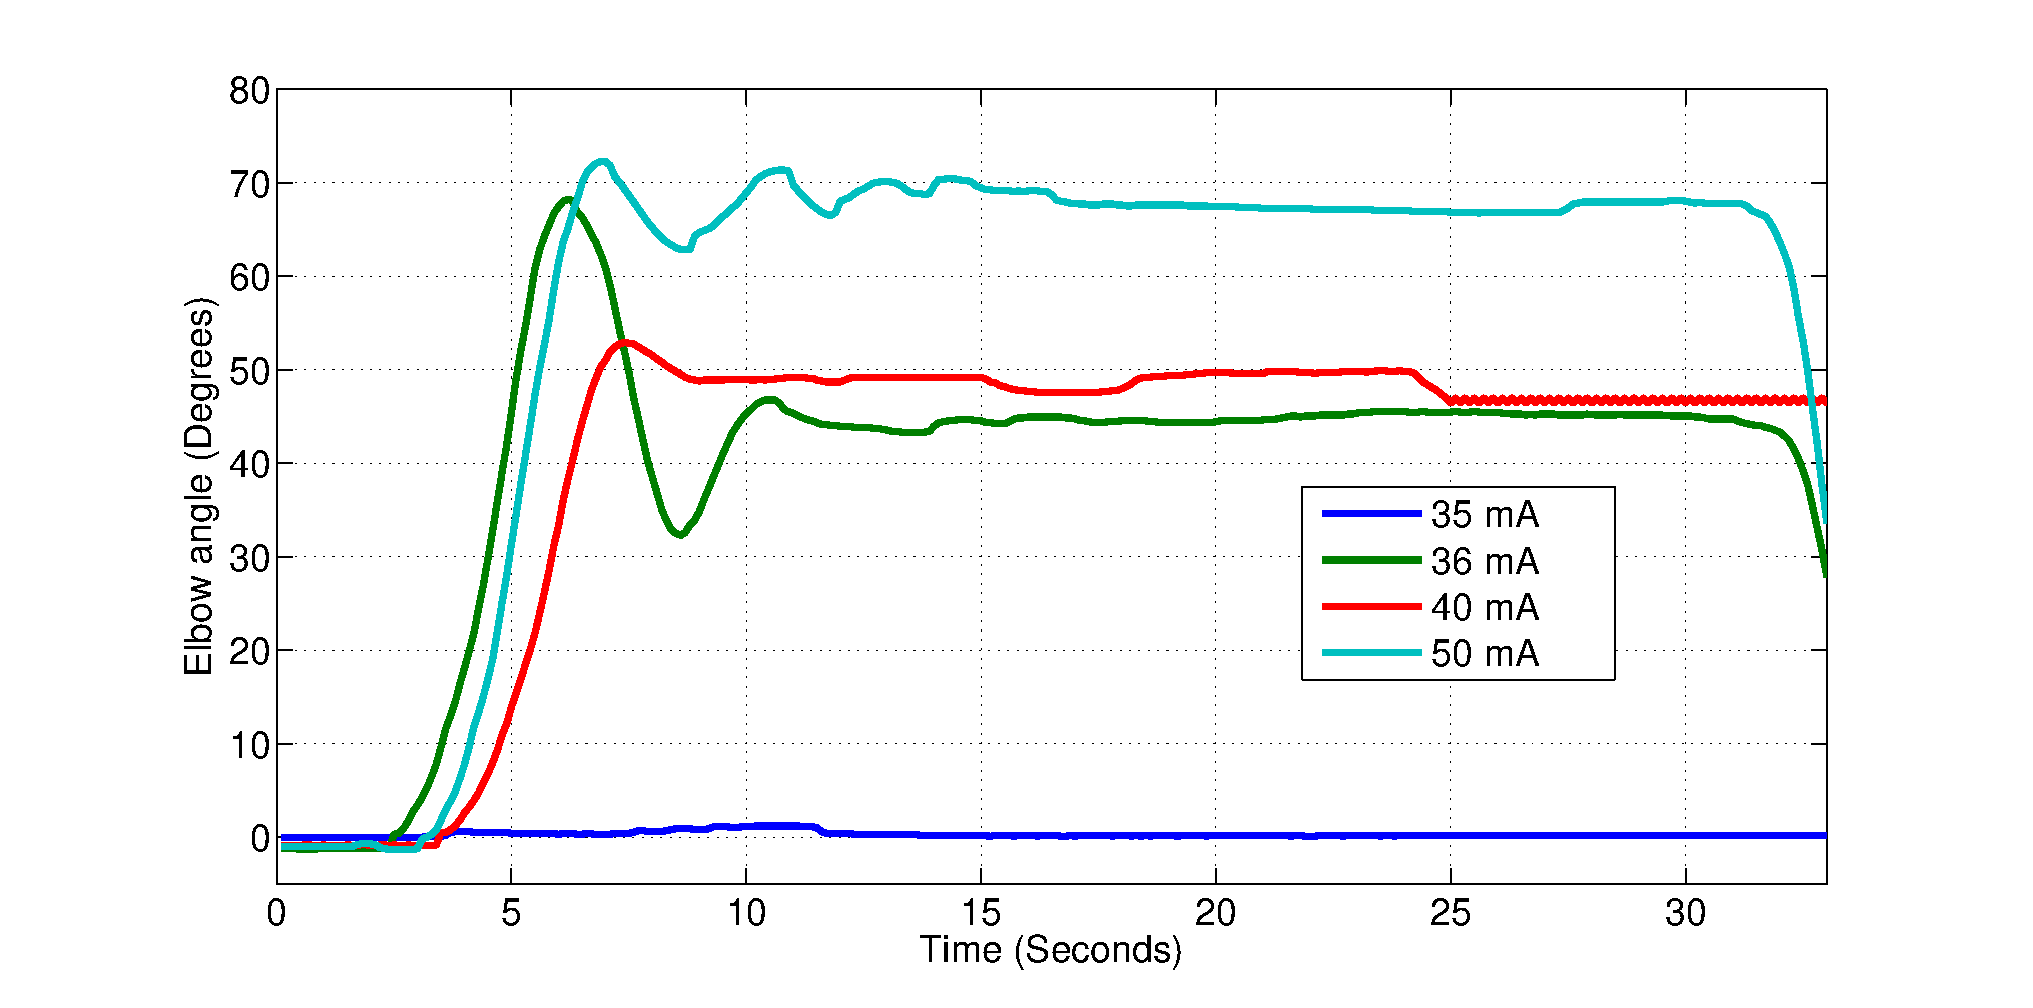
\includegraphics[width=10.5cm]{todas_new.eps}
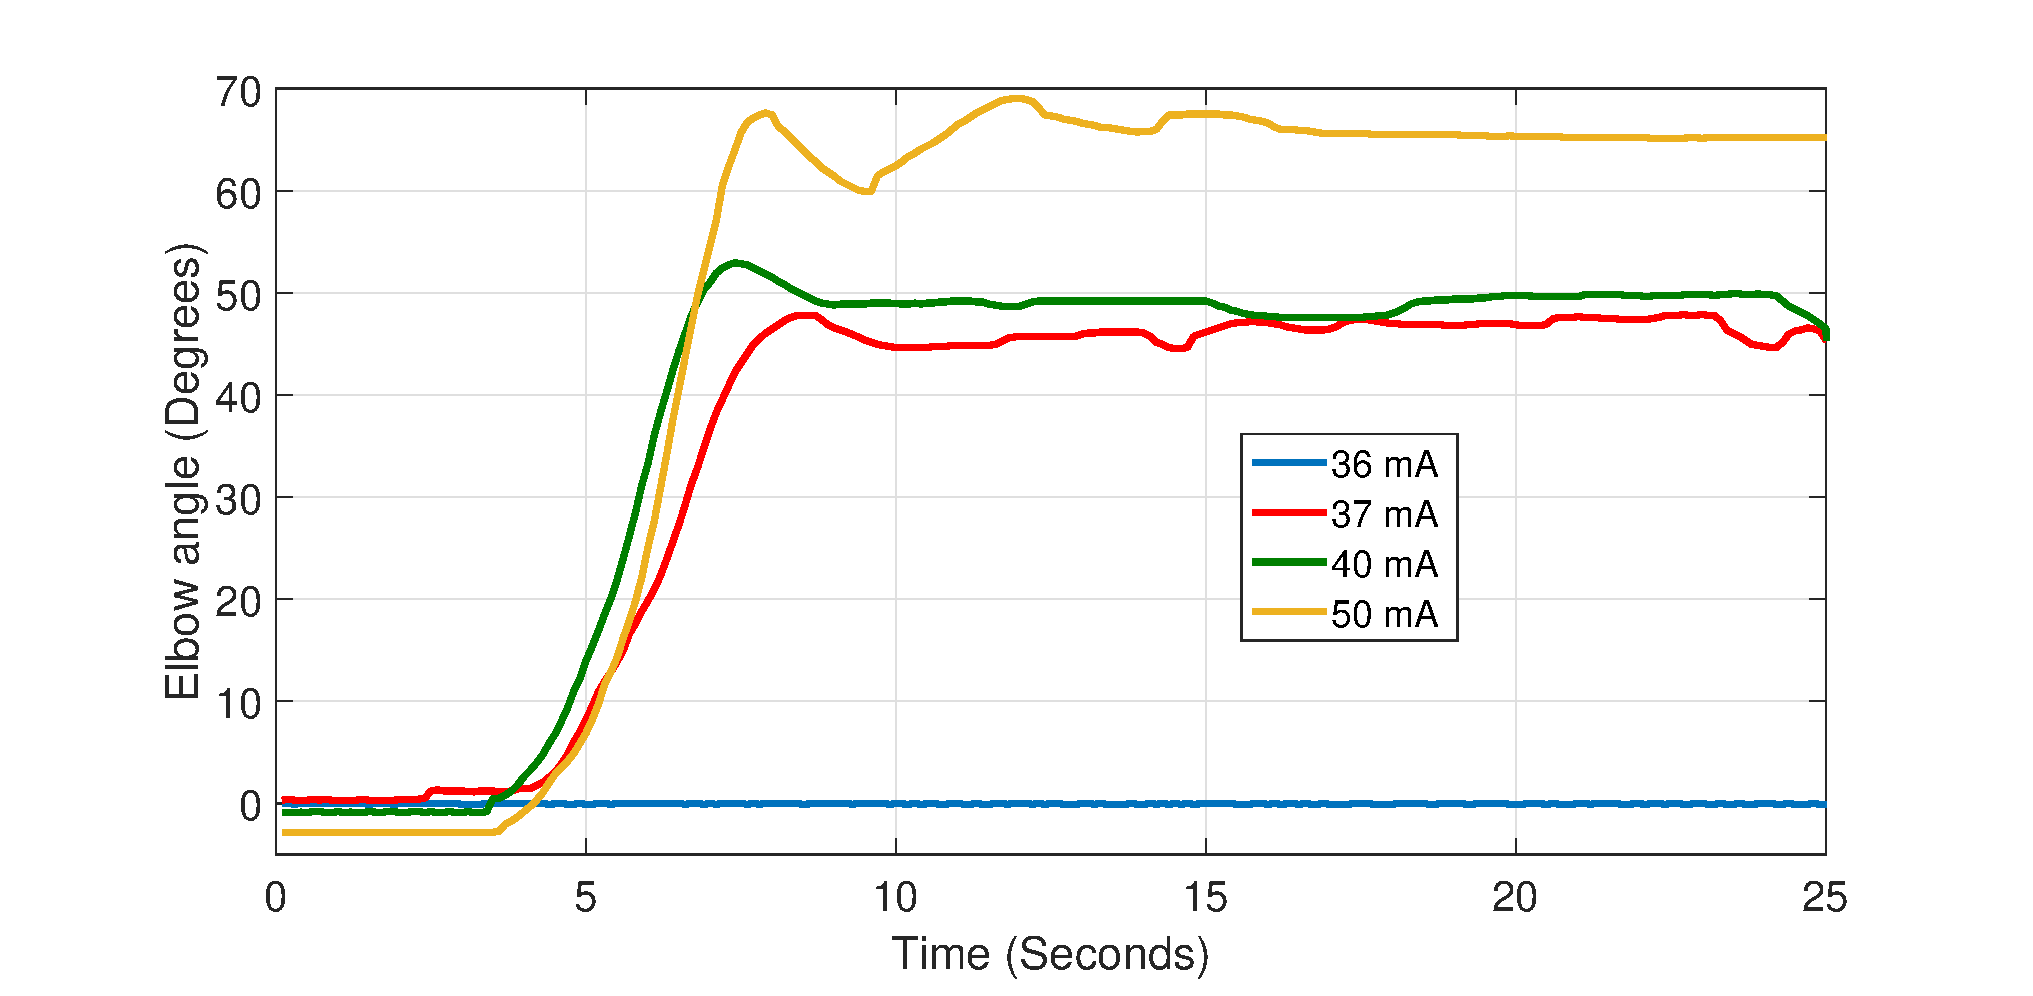
\includegraphics[width=12cm]{fig3.eps}
\caption{Results obtained in open-loop tests for the same volunteer: four different values of step current inputs at initial time
$t_0=3\ $s.}
\label{fig5}
\end{center}
\end{figure}
%
\begin{figure}[!htb]
%\hspace{-0.8cm}
\begin{center}
%\includegraphics[width=.44\textwidth]{Figures/fig5.eps}
%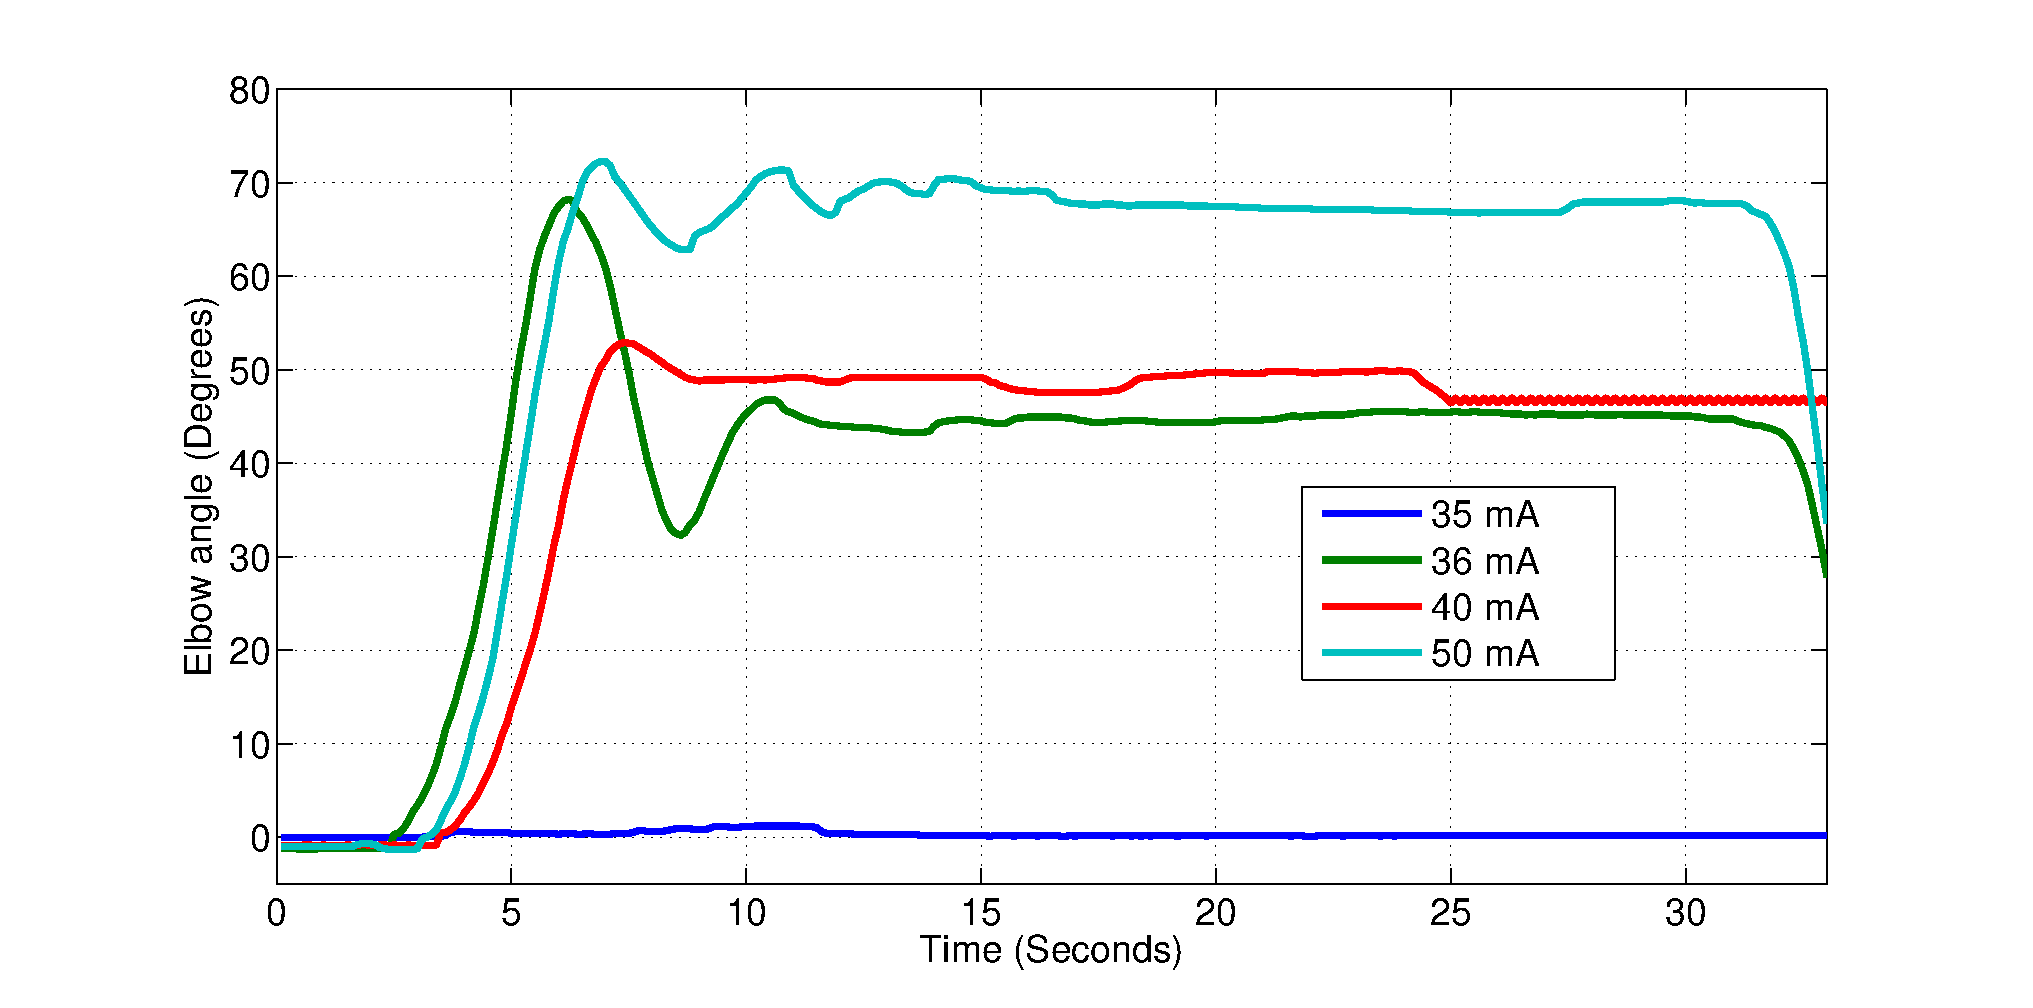
\includegraphics[width=10.5cm]{todas_new.eps}
%\includegraphics[width=12cm]{ma1.eps}
\includegraphics[width=13cm]{MalhaAberta2}
\caption{Results obtained in open-loop tests for the same volunteer: the same step current inputs of $40$mA applied into different
time-instants.}
\label{fig50}
\end{center}
\end{figure}





\textcolor{black}{Therefore, the collection of open-loop responses shows} that the considered system behaves, or can be approximated to each stimulus, as a linear second order system with transport delays \cite{N:2009} and parametric uncertainties:
%
\begin{eqnarray}\label{plant}
H(s)=\frac{y}{u}=\frac{\textcolor{black}{K_{HFG}} ~e^{-D s}}{s^2+2\xi w_n s+w_n^2}\,,
\end{eqnarray}
%
where the constant \textcolor{black}{$K_{HFG}>0$} is the high-frequency gain, \textcolor{black}{$\xi>0$} is the
\textcolor{black}{damping ratio}, $w_n>0$ is the natural frequency of the model and $D \geq 0$ is a constant delay. The scalar signals $y(t)$ and $u(t)$ are the output angle of the elbow's arm (in degrees) and the electrical current stimulus input
(in mA), respectively. \textcolor{black}{By assumption, we are considering that any eventual canceling of zeros and poles in (\ref{plant}) with negative real parts would be even possible, resulting in a non-minimal state-space which is still ISS.}




All parameters of \textcolor{black}{the system} can be assumed unknown but belonging to a bounded range of uncertainty.
%that is used in the controller design.
In the open-loop experiments of Figure~\ref{fig5}, the parameters have varied within the following ranges:
%
\begin{eqnarray}
0.012 \ <  \!\!\!\! &\textcolor{black}{K_{HFG}}& \!\!\!\! < \  0.019 \,, \label{shit1}\\
0.007 \ < \!\!\!\! &2\xi w_n& \!\!\!\! < \ 0.29\,, \\
0.001 \ < \!\!\!\! &w_n^{2}& \!\!\!\! < \ 0.02\,, \\
0.3 \ < \!\!\!\! &D& \!\!\!\! < \ 0.8\,. \label{shit2}
\end{eqnarray}
%
\textcolor{black}{The parameters in (\ref{shit1})--(\ref{shit2}) can be easily obtained from the responses in Figure~\ref{fig5} by applying 
the fitting procedure for curves of the \textcolor{black}{\textit{System Identification Toolbox} 9.2 for MATLAB (Mathworks, USA).}}

\textcolor{black}{The curves in Figure~\ref{fig5} and the parameters in (\ref{shit1})--(\ref{shit2}) are merely illustrative. In other words, the parameters values and their statistical distribution will be irrelevant to the demonstration of the stability properties for the closed-loop system, once it is only assumed that the plant is ISS. The presented model could be clearly fitted by a nonlinear second order system. \textcolor{black}{However,} the system parameters are different for each volunteer, and their correct identification is not an easy task to be done in clinical procedures, where the same controller is applied to different patients with distinct kinds of lesion. Therefore, controllers that require a precise model of the plant are not suitable for such an application.}

\newpage


\section{\textcolor{black}{Control Objective and Experimental Protocol}}


The aim is to develop a control law based on output feedback to drive the angular error defined by 
%
\begin{eqnarray}\label{error}
e(t)=y(t)-y_m(t) 
\end{eqnarray}
%
to a small neighborhood of zero, where the output $y$ given in (\ref{plant}) is the elbow's arm (joint) angle measured by a goniometer
and $y_m$ is the desired reference angle. \textcolor{black}{A block diagram of the proposed control system for NMES is illustrated in Figure~\ref{supercoco}.} 
%%
\begin{figure}[!htb]
%\hspace{-0.5cm}
%\begin{center}
%\includegraphics[width=.44\textwidth]{Figures/fig50.eps}
%\includegraphics[width=10.5cm]{rele_new.eps}
\includegraphics[width=12cm]{FigI2.pdf}
\caption{\textcolor{black}{Block Diagram of the closed-loop system for NMES.}}
%\caption{Resposta $y$ paciente e sinal de referência $y_m$.}
\label{supercoco}
%\end{center}
\end{figure}


In our experiments, \textcolor{black}{the muscles are electrically
stimulated to provide a unilateral movement of the arm} of the volunteer
in order to track the reference angle. For such an electrical stimulation,
both control channels stimulating biceps and triceps muscles must
be used. \textcolor{black}{The idea is very intuitive. Since the system
in question is always positive \cite{FR:2000} (the system variables
}\textcolor{black}{do not} assume negative values), the control signal
is divided in two: positive and negative part. \textcolor{black}{The
former is applied to the biceps, generating upward movements, while
the latter, when applied to the triceps, generates downward movements.}


\textcolor{black}{In theory, the triceps activation would be barely
needed for healthy volunteers since gravity naturally }\textcolor{black}{causes}
an extension of the arm, bringing it back toward zero (relaxed position).
However, during an extension movement, the TB may be active, \textcolor{black}{which
has an effect on the rate of extension} and once the arm has already
achieved the desired set point, this term will be very important to
compensate small errors (fluctuations) around the desired position,
thus allowing a less aggressive control action. In addition, it is
worth mentioning that the triceps activation would be crucial for
stroke patients once gravity component is not enough to force the
injured arm in following the desired movement/trajectory.


\textcolor{black}{During the test protocol, experimental data were
collected with blindfold healthy volunteers and
collaborative stroke patients. It is worth mentioning that the healthy 
volunteers do not know the target (reference) angle for the elbow,
but the perception of the muscle stimulation is clear for them. It
means that the volunteers know which muscle (biceps
or triceps) is being stimulated and when the controller is actuating.
The most important condition is that the volunteer needs
to be relaxed and apart of the desired trajectory for the movement
in order to minimize their active participation. Stroke
patients were instructed to follow a visual feedback signal with a desired
trajectory. The reference trajectory is composed by a set of three  elbow
flexion-extension movements, which are performed with the
PI controller and another round with the sliding mode controller in order 
to avoid that healthy volunteers learn the proposed movement. A rest of at least five
minutes between each set was allowed to the subjects. The controllers were
applied in a random sequence. In addition to the \textbf{unilateral
movements} produced with the reference signal generator mentioned
above, homologous contralateral joint angle control will also be explored
for \textbf{bilateral symmetrical motion} tests \cite{SFYLS:2012}.}

\textcolor{black}{As a metric to evaluate the improvement of the proposed controller over PI controller, the RMS error of the trajectory was compared for both cases using Wilcoxon signed rank test, a non parametric statistical  hypothesis test to compare small groups with repeated samples.}



\section{\textcolor{black}{Sliding Mode Control via Time-scaling}}


In order to obtain a control strategy robust to modeling uncertainties, but
simpler than the current nonlinear controllers used for NMES (e.g., see \cite{BFF:2015}, \cite{FHBC:2009}), \textcolor{black}{we will combine principals of both time-scaling and sliding mode control.} 

The proposed strategy is applicable to a wide class of plants with uncertain and arbitrary relative degree. A limitation of the time-scaling procedure is that it is restricted to stable systems. However, this is not a problem since the neuromusculoskeletal model considered here satisfies such an assumption. By using singular perturbation methods, it is shown that in a new time scale the considered system can be reduced to a simple integrator perturbed by a rapid sensor dynamics, which in turn ultimately converges to a small residual set.


Then, we exploit this particular structure to redesign our sliding mode control law to show its robustness
with respect to the arbitrary relative degree dynamics at expense of some time dilation, which slows
down the system response.




\subsection{Background}

Consider the following linear system:
%
\begin{eqnarray}
    \dot v &=& u \,,      \label{eq0}\\
    \dot{x}&=& Ax+Bv \,,  \label{eq1}  \\
    y&=&Cx \,,            \label{outupunmeasured}
\end{eqnarray}
%
where $x \in
\mathbb{R}^n$ is the unmeasured state vector, $u \in \mathbb{R}$ is the control input, $y \in \mathbb{R}$ is system output
and the relative degree of the subsystem $(A,B,C)$ is \textcolor{black}{denoted by $n^*$.} 
%
\begin{remark}
\textcolor{black}{\textit{Chattering} is a typical but undesirable phenomenon that arises in all sliding mode controllers due to the high-frequency nature of the switching actuator \cite{UGS:99}. The source of chattering in sliding mode control schemes are distinct and coexistent: numerical discretization, switching delays, unmodeled dynamics, measurement noise, etc.} 
The integrator in (\ref{eq0}) is used to obtain a virtual control signal
$v \in \mathbb{R}$, which increases the relative degree of the overall system \cite{Lev:03}, \textit{i.e.},
$n\geq n^*-1$ instead of $n\geq n^*$. The increase of the relative degree retains the high-frequency switching to the control signal $u$,
whereas the virtual control $v$ that directly drives the plant is continuous.
Thus, it is expected that the effects of chattering in the proposed sliding mode controller can be attenuated.
%
\end{remark}


\textcolor{black}{The relative degree is a mathematical concept in nonlinear control theory which measures how \textcolor{black}{many times} the output of a system must be differentiated so that the control input can be found \cite{K:2002}. For linear systems, 
the relative degree of a rational transfer function $$G(s)=N(s)/D(s)=C(SI-A)^{-1}B$$ is $n^*=\text{deg}(D(s))-\text{deg}(N(s))$, \textit{i.e.}, the difference between the number of poles and zeros of the transfer function. For a proper
transfer function, the relative degree is a nonnegative integer.} \textcolor{black}{Indirectly, the relative degree indicates the degree of complexity in controlling a given system. In general, for higher relative degrees, the control design will demand higher-order differentiation \cite{L:2000}, which is not the focus of our strategy.}





\textcolor{black}{
Since the neuromusculoskeletal models used in NMES are uncertain in order or not perfectly known, the relative degree is uncertain or
unknown as well. It can be easily verified when we (and other authors in the literature) approximate the real system by \textcolor{black}{an} ISS second order model. In our case, we also approximate the delay term by rational complex functions by Pad\'e operators with order strictly dependent on the delay size. In \textcolor{black}{these} cases, model inaccuracies can lead to the increase/decrease of the
relative degree.} Thus, the constant matrices $A\in\mathbb{R}^{n\times n}$, $B\in\mathbb{R}^{n}$, $C\in\mathbb{R}^{1\times n}$, the order $n$ of the subsystem (\ref{eq1}) and, consequently, the relative degree $n^*$ are \textit{all assumed uncertain}. In particular, the matrix $A$ must be Hurwitz.

\textcolor{black}{From Section~\ref{empirical}, the triple $(A, B, C)$ is assumed constant for each muscle group (biceps or triceps), but uncertain and belonging to some compact set. The basic idea is to show that for each input the system response could be roughly approximated by a second order delayed linear system subject to order variations and parametric uncertainties
(e.g., $A=A_0 + \Delta_A$, where $A_0$ is some known nominal value and $\Delta_A$ represents the parametric uncertainty in $A$, satisfying
$||\Delta_A||\leq K_A$ with $K_A>0$ and $||\cdot||$ denoting induced norm of matrices).}
%
\emph{A priori}, the triple $(A,B,C)$ can be used to represent the state-space representation
of the transfer function (\ref{plant}). Nevertheless, the system has a delay which can be handled by using a Pad\'{e} approximation obtained through the expansion of irrational function $e^{-D s}$ \textcolor{black}{into a rational function whose numerator and denominator are polynomials with degree $p$, %and the denominator has degree $q$,
see \cite{L:1990} and references therein: 
%
\begin{equation*}
e^{-D s}\approx \frac{1 - k_1 s + k_2 s^2 + \ldots \pm k_p s^p}{1 + k_1 s + k_2 s^2 + \ldots + k_p s^p}\,,
\end{equation*}
%
\textcolor{black}{where $p$ is the order of the approximation. The coefficients $k_i$ are functions of $D$.} 
%%
%For example, if $p=2$, we have:
%%
%\begin{eqnarray*}
%e^{-D s}\approx\frac{1-(D s)/2+(D s)^2/12}{1+(D s)/2+(D s)^2/12}\,,
%\end{eqnarray*}
%%
%and if $p=1$, we get:
%\begin{eqnarray}\label{delay0}
%e^{-D s}\approx\frac{1-(D s)/2}{1+(D s)/2}\,.
%\end{eqnarray}
%}
%%
%In some cases, a very crude approximation is also acceptable.
%\textcolor{black}{For very small delays, even the following simple first-order lag approximation} can be made \cite{FPE:2009}:
%%
%%Para sistemas com atrasos muitos pequenos, a seguinte aproximação
%%trivial pode ser feita \cite[]{FPE:2009}:
%%%
%\begin{eqnarray}\label{delay1}
%e^{-D s}\approx\frac{1}{1+D s}\,,
%\end{eqnarray}
%%
%\textcolor{black}{which also justifies the robustness of the proposed controller to unknown delays, since they may be implicitly included in the stable dynamics of the triple $(A,B,C)$ in (\ref{eq1})--(\ref{outupunmeasured}).
%
For longer delays, higher order Pad\'{e} approximations can be adopted \cite{L:1990}. Since all rational Pad\'e approximations for the irrational term $e^{-Ds}$ return stable transfer functions
(possible non-minimum phase), the only information we must know is that the delay is bounded. }


\textcolor{black}{Basically, we replace the delay term $e^{-Ds}$ by some rational and stable complex function of the complex variable $s$ which sufficiently approximates the original term for a given order $p$ and so that it can be also encompassed in the dynamics described in
(\ref{eq1}). After the application of the time-scaling procedure introduced in the next section, such terms can always be faced as a unmodeled dynamics for (\ref{eq0}),  if $\mu$ is sufficiently small.}

Differently from the predictor-based approaches to delay compensation \cite{SGD:2011}, \cite{KMQKY:2014}, which are highly dependent
on the order of the plant model and its parameters knowledge, we use the approximation above of any order to simplify the control design in the next section. \textcolor{black}{In practice, the influence of such an approximation order in the control design is verified by the magnitude of the parameter $\mu$ of the time-scaling, that is: longer delays demand higher-order Pad\'e approximation, \textcolor{black}{which implies} smaller $\mu$'s. \textcolor{black}{Despite this} tied relation, the latter can be tuned without the exact knowledge of the delay and the order of the Pad\'e operator either, as will be shown.}



\subsection{Time-scaling for control design}
\label{coco}

\textcolor{black}{The main theoretical contribution of the present paper is to propose a control design which is independent of the knowledge of the relative degree, supposing the plant possesses some ISS properties. The practical motivation of the problem is then illustrated and evaluated in the functional electrical stimulation scenario. To the best of our knowledge, this methodology was not considered before and can bring advantages in practice, such as the avoidance of a lengthy identification or tuning procedures for NMES treatment sessions.
\textcolor{black}{Nonetheless,} any unpredictable rapid variation in the system could change the representative model and model order variations could degrade the performance of the treatment.}


In \cite{UGS:99}, it was shown that sliding mode controllers based on high-gain relay feedback can be designed to the tracking problem for plants with unitary relative degree ($n^*=1$). Here, we show that this \textcolor{black}{class of compensator} can be extended to the arbitrary relative degree case and applied to NMES \text{black}{as well.} 

In order to present such a generalization, consider the simplest integrator dynamics with input $u$ and output $y$:
%
\begin{eqnarray}
  \dot v &=& u\,,   \label{unitary_plant_inverse2}\\
  y&=& Cv\,,    \label{unitary_saidameasured}
\end{eqnarray}
%
which can be easily controlled by the first order sliding mode approach introduced  in \cite{UGS:99}.



By using the singular perturbation method \cite{K:2002},\cite{KKO:1986}, \cite{U:92} it is possible to show that sliding mode controllers are indeed robust to fast unmodeled dynamics such that the perturbed system (\ref{unitary_plant_inverse2})--(\ref{unitary_saidameasured}) can be  rewritten in the following canonical \textit{block sensor form}
\cite[p.50]{KKO:1986}:
%
\begin{eqnarray}
    \dot v &=& u \,,                               \label{fast_eq0}\\
    \mu\dot{x}&=& Ax+Bv \,,                        \label{fast_eq1}  \\
    y &=& C x \,,                            \label{fast_outupunmeasured}
\end{eqnarray}
%
and satisfies the inequality
%e satisfaz a inequação
%%
\begin{eqnarray}
    |y-y_m| \leq \mathcal{O}(\mu)\,,    \label{residual_set}
\end{eqnarray}
%
after a transitory phase, since $\mu>0$ is a sufficiently small constant. The demonstration of this result follows similar steps given in the stability analysis in Appendix~A.  


\textcolor{black}{In order to clarify the notation to the reader, as defined in \cite{KKO:1986}, we say that a vector function $f(t,\mu) \in \mathbb{R}^n$ is of order $\mathcal{O}(\mu)$ over an interval $[t_1\,, t_2]$ if there exist positive constants $k$ and $\mu^*$ such that $|f(t,\mu)| \leq k \mu$,  $\forall \mu \in [0,\mu^*]$ and $\forall t \in [t_1,t_2]$. In some cases, we will be able to give estimates of constants $k$ and $\mu^*$ and thus quantify the corresponding $\mathcal{O}(\mu)$ approximations. Otherwise, we will be satisfied by $\mathcal{O}(\mu)$ being an ``order of magnitude relation'', valid for ``$\mu$ sufficiently small''.}


By applying the following linear time-scaling \cite{MONPP:2002}
%
\begin{equation}
  \frac{d t}{d \tau} = \mu\,,                                              \label{time-scaling}\\
\end{equation}
%
we can rewrite the system (\ref{fast_eq0})--(\ref{fast_outupunmeasured}) into
%
\begin{eqnarray}
  v' &=& \mu u\,,           \label{eq02}\\
  x' &=& A x + Bv\,,     \label{plant_inverse2}\\
  y&=& Cx\,,         \label{saidameasured}
  \end{eqnarray}
%
where $v':=\frac{d v}{d \tau}$ and $x':=\frac{d x}{d \tau}$. This means that $\exists \mu^*>0$ such that the input signal $u$
can be scaled (\ref{eq02}) to control the original system (\ref{eq1})--(\ref{outupunmeasured}) on a different dilated time scale given by %$t=\mu\tau$, $\forall \mu \in (0,\mu^*]$.
%
$\tau=(t-t_0)/\mu$,  $\forall \mu \in (0,\mu^*]$, and $t_0$ being any arbitrary initial time.


\textcolor{black}{The time-scaling (\ref{time-scaling}) is indeed indirectly applied to the system (\ref{eq0})--(\ref{outupunmeasured}) and the latter is transformed to (\ref{eq02})--(\ref{saidameasured}). Both systems are equivalent in the different time scales $t$ and $\tau$, respectively.} 
%
\textcolor{black}{The physical meaning of the proposed time-scaling procedure is: if a sliding mode controller originally proposed for a relative degree one system (in our case a simple integrator (\ref{unitary_plant_inverse2})--(\ref{unitary_saidameasured})) is robust to fast and stable unmodeled dynamics as the parameter $\mu\to+0$, then the same controller is suitable for controlling systems with arbitrary relative degree dynamics, if it is properly scaled \cite{HOC:2014}, \cite{OAH:2014}. As expected, the price to pay is that the system response in closed loop slows down as $\mu\to +0$.}



\subsection{The singular case: $\mu=0$}

In this case, the differential equation (\ref{fast_eq1}) is replaced by the algebraic equation $x=-A^{-1}Bv$. From
(\ref{fast_eq0}) and (\ref{fast_outupunmeasured}), the first derivative of the output signal $y$ with respect to time is given by
%
\begin{align}
\dot{y} = K u\,,\label{eq:ydynamics}
\end{align}
%
where the high frequency gain $K$ is given by
%
\begin{align}
K=-CA^{-1}B\,. \label{kpneras}
\end{align}


From (\ref{error}) and (\ref{eq:ydynamics}), the time derivative of the error $e(t)$ is given by
%
%
\begin{align}
\dot{e}&=K u- \dot y _m\,, \\
\dot{e}&=K(u+d_e)\,, \label{edoerro}
\end{align}
%
with
%
\begin{align}
d_e:=-\dot y _m/K \,. \label{moduerro}
\end{align}

By using the Lyapunov function $V(e)=e^2/2$, \textcolor{black}{it can be shown} that if the control law
%
%
\begin{align}\label{amor}
    u=-\sgn(K)\rho\sgn(e)
\end{align}
%
is used with a non-negative \textcolor{black}{\textit{modulation function}} $\rho$ satisfying
%
\begin{align}
\rho(t)\geq|d_e(t)|+\delta, \label{funcmodgen}
\end{align}
%
and $\delta\!>\!0$ being any arbitrary small constant, then using the \textit{Comparison Lemma} (Appendix B), we have the
tracking error $e(t)$ converging to zero in finite time, \textit{i.e.},
%
\begin{equation}
e(t)=0\,, \quad \forall t
> t_{s1}\,,
\label{eq:boundMIMOKpconhecido2}
\end{equation}
%
for some finite time $t_{s1}>0$.
%
%sendo $t_{s1}>0$ algum instante de tempo finito.

\textcolor{black}{Note that we need only to know the sign of $K$ in (\ref{amor}), not its value. Since it can only be negative or positive, a simple trial test solves it. The sign of $K$ is related to the negative feedback or control direction for the closed-loop system. In general, it is assumed known in almost every control system.}

One possible choice for the modulation function to satisfy (\ref{funcmodgen}) is given by
%
\begin{align}
\rho(t)=\bar{d}_e(t)+\delta, \label{funcmodgenequal}
\end{align}
%
where $\bar{d}_e(t)=\bar{k}_m(t)/\underline{k}$ is a known upper bound for $|d_e(t)|$. The signal $\rho(t)$ is constructed with any constant lower bound $\underline{k}$ for $K$ in (\ref{kpneras}), considering all the admissible uncertainties in ($A$, $B$, $C$), \textit{i.e.},
%
\begin{equation}
0<\underline{k}\leq|-CA^{-1}B|\,,
\end{equation}
%
and $\bar{k}_m(t)$ being a valid upper bound
%
\begin{equation}
|\dot{y}_m| \leq\bar{k}_m(t)\,,
\end{equation}
%
for the time derivative of the desired trajectory $y_m(t)$.


\subsection{Controller scaled parameters: $\mu \neq 0$}

When $\mu\neq 0$ in (\ref{fast_eq1}), the time scale (\ref{time-scaling}) \textcolor{black}{allow us to} consider the original plant
(\ref{eq1})--(\ref{outupunmeasured}) in a different time scale being controlled by the controller (\ref{amor})
properly scaled by $\mu u$, see (\ref{eq02}). In order to incorporate it, the modulation function must be redesigned to satisfy
%
%
\begin{align}
\rho(t)=\mu[\bar{d}_e(t)+\delta], \label{fast_funcmodgen}
\end{align}
%
instead of (\ref{funcmodgenequal}).
%em vez de (\ref{funcmodgen}).

The analysis by means of singular perturbations shows that practical tracking can be obtained in the sense that the tracking error converges in finite time for a residual set of $\mathcal{O}(\mu)$ if $\mu$ is sufficiently small, \textit{i.e.},
%
\begin{equation}
|e(t)|\!\leq\!\mathcal{O}(\mu)\,, \quad \forall t>t_{s2}\,,
\end{equation}
%
where $t_{s2}>0$ is some finite time.
%


\textcolor{black}{The main stability results of the closed-loop system in Figure~\ref{supercoco} are stated in the Theorem~\ref{theorem1} given in Appendix~A.} 


 \textcolor{black}{In this manuscript, a linear approximation was used considering that the nonlinearities could be approximated rationally by elevating the order of the model, but maintaining the necessary and behavioral conditions of the plant (basic assumptions) for control design. According to Theorem~\ref{theorem1}, the local stability of the system can always be guaranteed using an appropriate value of $\mu$, such that the time-scaling makes the system to behave like a point-wise linear and invariant system, neglecting any errors from the approximation.}  \textcolor{black}{Furthermore, we just have one control signal $u(t)$ which is considered in the stability analysis and this same signal is used to control biceps and triceps. The biceps and triceps can be faced as a unique bidirectional actuator with hybrid dynamics, where the positive control signal is applied to biceps and its negative portion to triceps. The differences in biceps and triceps responses can be absorbed in the analysis by the uncertainties in the plant model (including the actuator). The overall analysis of this closed-loop hybrid system (that exhibits both continuous and discrete dynamic behavior) is out of the scope of the present article.}


%The control of systems with uncertain relative degree is a challenging task \cite{L:2012}, \cite{HFLSLMA:2013}. Here, this result is achieved %without the use of differentiators or observers \cite{Lev:03}, \cite{AFL:2012}, \cite{FSEY:2008}, \cite{BFU:1998}, \cite{OPH:2013}. The %time-scaling procedure is introduced to do this job by reducing the order of the system dynamics and thus allowing the analysis and the %control design for enlarged uncertainty in the relative degree in a simple way.


\textcolor{black}{
\begin{remark}
By utilizing a small $\mu$, the convergence rate of the control algorithm may become slow. However, it is always possible to consider an additional control term $u^*$ which accelerates the closed-loop dynamics so that the parameter $\mu$ in the proposed time-scaling based SMC law is not required to assume very small values. In this case, the SMC term acts like \textcolor{black}{a} robust adaptation element of the controller in order to correct errors due to parametric uncertainties, unmodeled dynamics and any kind of variation from different patients. Notice that it does not affect the proof of the stability results of Theorem~\ref{theorem1} since the term $u^*$ 
can be seen as the control law of an internal feedback loop which transforms the dynamics of the original plant into a faster one to be controlled by the SMC term. Formally, the control law would be given by
%
\begin{eqnarray} \label{cococococo1}
\dot v = -\sgn(K)\rho\sgn(e) \,, \\
u(t)=u^*(t)+v(t) \,, \label{cococococo2}  
\end{eqnarray}
%
with $\rho$ defined in (\ref{fast_funcmodgen}), and term $u^*$ transforms the original plant (\ref{eq0})--(\ref{outupunmeasured}) into the system 
%%
\begin{eqnarray}
    \dot v &=& -\sgn(K)\rho\sgn(e) \,,      \label{eq0_salvation}\\
    \dot{\bar{x}}&=& \bar{A}\bar{x}+\bar{B}v \,,  \label{eq1_salvation}  \\
    y&=&\bar{C}\bar{x} \,,            \label{outupunmeasured_salvation}
\end{eqnarray}
%
where the triple $(\bar{A},\bar{B},\bar{C})$ does not violate any of the original assumptions, but possesses a faster dynamics under the action of $u^*$. One possible choice for the auxiliary term $u^*$ is the PI control law, i.e.,
%%
\begin{eqnarray} \label{PID}
    u^*(t) &=& K_P ~e(t) + K_I\int_{0}^{t} e(\theta)~ d\theta \,, \quad \forall t \geq 0 \,,
\end{eqnarray}
% 
\end{remark}
where the constants $K_P$ and $K_I$ are the proportional and integral gains, respectively, satisfying $\sgn(K_P)=\sgn(K_I)=-\sgn(K)$.
}



In the next section, the proposed control scheme is experimentally evaluated in a real functional electrical stimulation scenario.
%
%Na próxima seção, avaliamos experimentalmente o esquema de
%controle proposto no problema de eletroestimulação funcional.



\section{Experimental Results}



\textcolor{black}{Experimental results are presented in order to validate the proposed NMES controller within a statistical perspective by using RMS errors and following the protocol in Section~\ref{protocol}. A detailed discussion of the closed-loop responses are also provided.} \textcolor{black}{In the next two sections, all tests performed with healthy volunteers are given for the proposed NMES controller as well as the PI control strategy in order to facilitate the comparisons. At last, the proposed NMES controller is evaluated with stroke patients in Section~6.3.}



\subsection{Bilateral symmetrical motion}

\textcolor{black}{Bilateral symmetrical motion \cite{SFYLS:2012} is an important part of the physiotherapy for stroke patients.
%, being the final objective of our study.
In this case, the contra-lateral movement of the non-actuated arm is used to generate a time-varying reference angle for the arm to be stimulated. In a clinical scenario, the patients know the trajectory of the movement to be performed, but they cannot execute it by themselves. The electrical stimulation helps the patient to complete the movement and improve its rehabilitation via motor relearning.} 

\textcolor{black}{On the other hand, any reference trajectory generated by one arm can be unconsciously perceived by the controlled arm of a healthy individual. Since this kind of evaluation would bring nothing methodological conclusive in our scenario with healthy volunteers, our tests were performed, but only links for the videos of the experiments have been included. Despite this kind of movement \textcolor{black}{not being} the main focus of the paper, our movies show the proposed time-scaling based SMC defined in (\ref{amor}) and (\ref{funcmodgenequal}) achieves the control objectives but may impose a very slow dynamics to the closed-loop system due to the time-dilation effect, which can be accelerated with the additional control term $u^*$ described in Remark~2.}


The videos of the experiments and the comparisons of the proposed strategy with a PI controller performing the tracking of the contra-lateral limb (right arm) can be found in the links below:
%
\begin{small}
\begin{itemize}
%
\item PI Control \\ \textcolor{blue}{\href{https://docs.google.com/file/d/0B8M1zh-nMf-kMm5Sc1JJX2NxVVU/edit}{https://docs.google.com/file/d/0B8M1zh-nMf-kMm5Sc1JJX2NxVVU/edit}} 
%
\medskip
%
\item Time-Scaling based Control \\ \textcolor{blue}{\href{https://docs.google.com/file/d/0B8M1zh-nMf-kejVwa29zNWRqV0U/edit}{https://docs.google.com/file/d/0B8M1zh-nMf-kejVwa29zNWRqV0U/edit}}\\
%
\end{itemize}
\end{small}


\subsection{Unilateral movements}

\textcolor{black}{Distinct (computed) reference trajectories are explored in the next experiments. For example, we have considered a trapezoidal reference with multiple cycles. In particular, the second derivative of the trapezoidal curve contain impulses which offer an \textcolor{black}{additional} challenge to the controller since it sets the desired angular acceleration of the elbow. In general, we only find in the literature of NMES sufficiently smooth trajectories (with smooth derivatives), which facilitates the tracking control problem. However, although we just have considered tests with healthy volunteers, it is worth mentioning that the final objective of our control application is for motor rehabilitation of stroke patients. The use of more sophisticated trajectories is not the focus in this kind of therapy, where simple and cyclic movements are applied to motor training. %The movements are restricted due to the mechanical parts of the apparatus and the electrical %stimulation is carried out recruiting only two main muscles group (biceps and triceps).
Despite the large number of research papers working on more complex control algorithms for producing coordinate movements, we can find few works focusing on physiotherapy. In this sense, the use of NMES oriented to physiotherapy until the occurrence of fatigue should be avoided in a real scenario since the idea here is motor relearning.}

\textcolor{black}{Eight volunteers with no orthopedic or neurological injuries were recruited. Prior to participation, written informed consent was obtained from the \textcolor{black}{individuals.} The plots of Figures~\ref{plot1} to \ref{plot4} present the movements for two representative subjects.} 

\textcolor{black}{In the next experiments, we implement the controller (\ref{cococococo1})--(\ref{cococococo2}) with $\rho$ defined in (\ref{fast_funcmodgen}) and $u^*$ being simply the PI control in (\ref{PID}). The constant modulation function is simply chosen as $\rho=\mu=0.01$ and the gains of the PI controllers are: $K_P=0.4$ and $K_I=0.2$. The control signal $u$ is saturated according to the discomfort of each volunteer. In what follows, we display the advantages of the time-scaling SMC term combination over a solely PI controller.}

The discrete implementation and quantization of the controller as well as the unmodeled dynamics present in the tests may induce the occurrence of \textit{chattering phenomenon} \cite{UGS:99}. However, this is not a problem since the switching term was filtered, being a smooth signal. This is guaranteed through the integral action in (\ref{eq0}) which is used \textcolor{black}{to reduce the chattering
\cite{FE:2014,AE:2009}}, one of the main drawbacks of the sliding mode controllers in real applications. Note that, when the biceps and triceps are active, the control signals are always greater than some minimal value (non-zero lower bound) due to the 
\textcolor{black}{dead-zone nature of the muscle actuator \cite{SNPHFFR:2005}}.

\newpage

\textcolor{black}{Figures~\ref{plot1} to \ref{plot4} %and \ref{fig53}
illustrate the robustness of our sliding mode control scheme calibrated for pretrial tests, but then applied to different volunteers in order to track trapezoidal reference signal. The response curves ratify the highly successful behavior of the proposed control scheme even in this adversary scenario for NMES.}
%%
\begin{figure}[!htb]
%\hspace{-0.5cm}
\begin{center}
%\includegraphics[width=.44\textwidth]{Figures/fig50.eps}
%\includegraphics[width=10.5cm]{rele_new.eps}
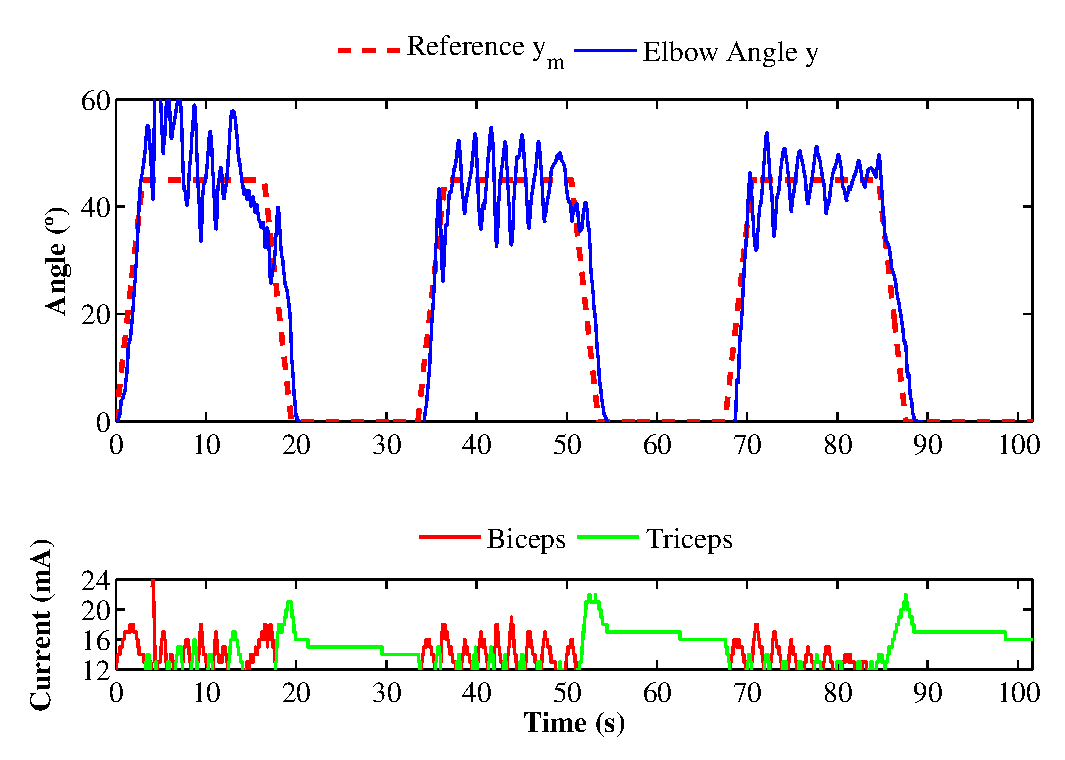
\includegraphics[width=12cm]{VIC1204PI.eps}
\caption{PI control (volunteer 1): response $y$ and reference $y_m$; control signal $u$.}
%\caption{Resposta $y$ paciente e sinal de referência $y_m$.}
\label{plot1}
\end{center}
\end{figure}
%
%
\begin{figure}[!htb]
%\hspace{-0.5cm}
\begin{center}
%\includegraphics[width=.44\textwidth]{Figures/fig50.eps}
%\includegraphics[width=10.5cm]{rele_new.eps}
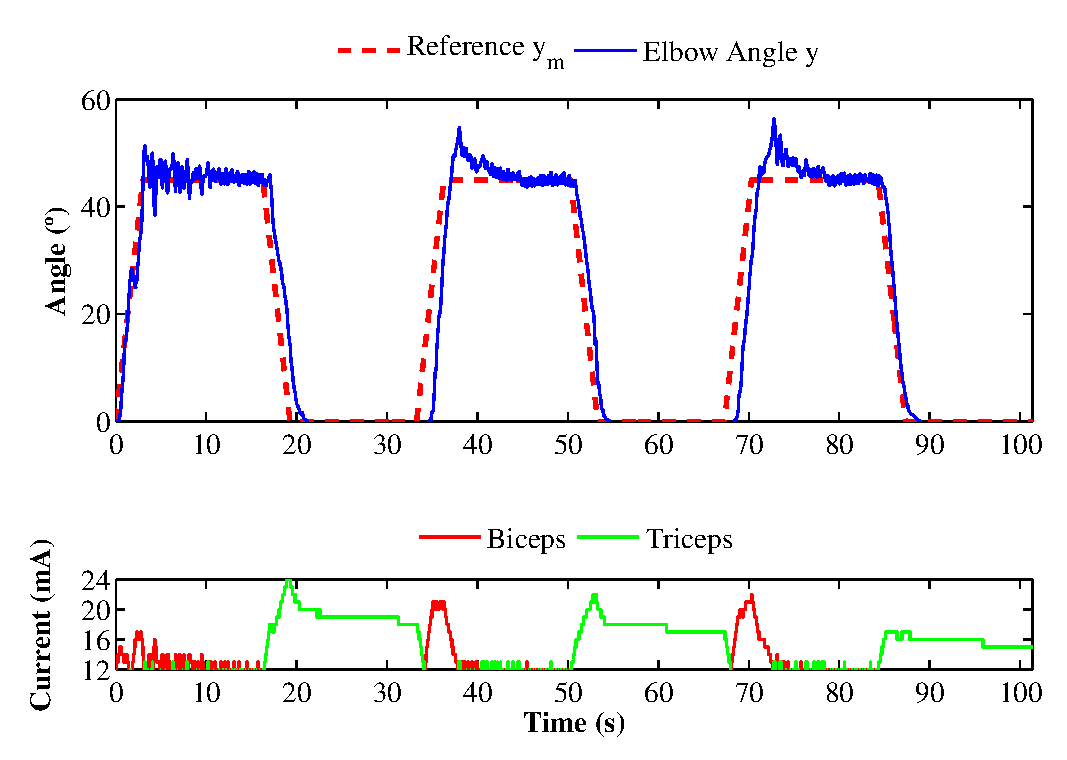
\includegraphics[width=12cm]{VIC1204PIRele.eps}
\caption{Time-scaling SMC (volunteer 1): response $y$ and reference $y_m$; control signal $u$.}
%\caption{Resposta $y$ paciente e sinal de referência $y_m$.}
\label{plot2}
\end{center}
\end{figure}
%
%%
\begin{figure}[!htb]
%\hspace{-0.5cm}
\begin{center}
%\includegraphics[width=.44\textwidth]{Figures/fig50.eps}
%\includegraphics[width=10.5cm]{rele_new.eps}
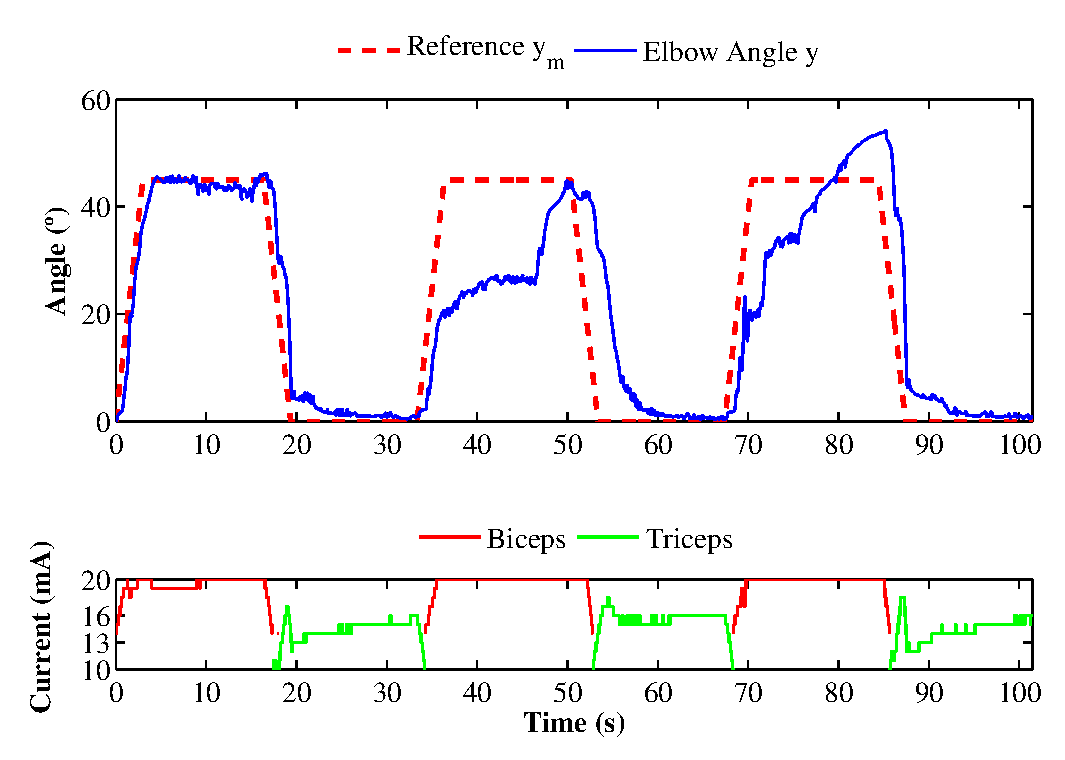
\includegraphics[width=12cm]{POV2604PI.eps}
\caption{PI control (volunteer 2): response $y$ and reference $y_m$; control signal $u$.}
%\caption{Resposta $y$ paciente e sinal de referência $y_m$.}
\label{plot3}
\end{center}
\end{figure}
%
%
\begin{figure}[!htb]
%\hspace{-0.5cm}
\begin{center}
%\includegraphics[width=.44\textwidth]{Figures/fig50.eps}
%\includegraphics[width=10.5cm]{rele_new.eps}
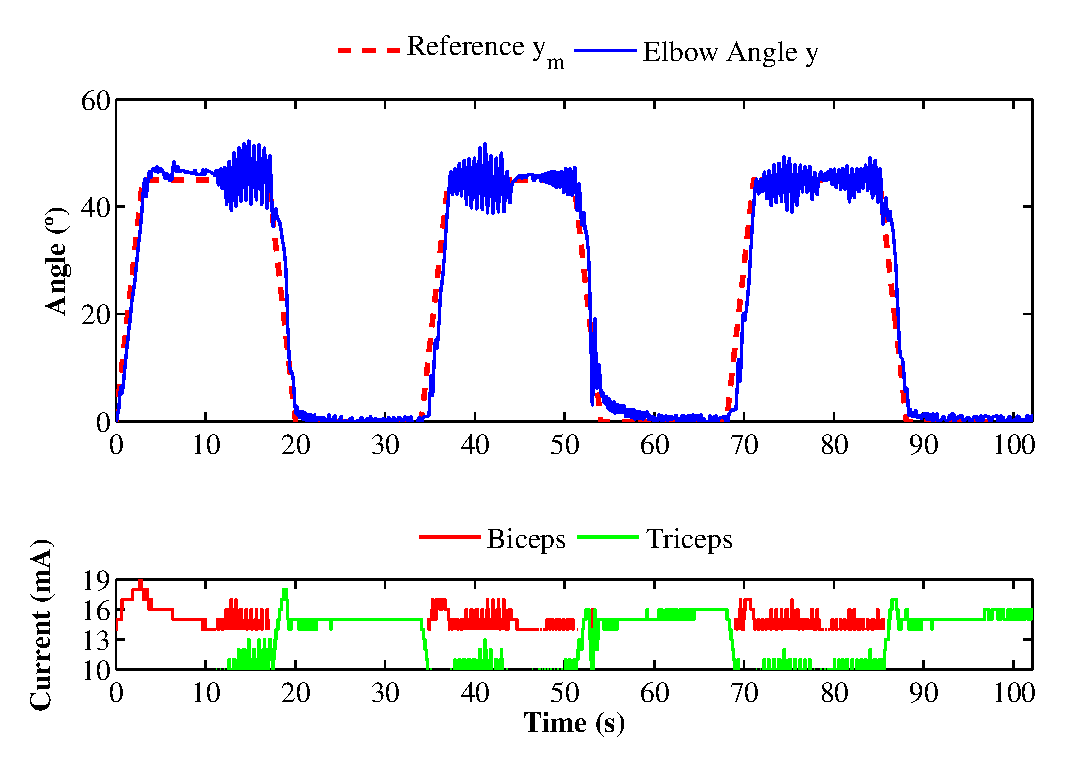
\includegraphics[width=12cm]{POV2604PIRele.eps}
\caption{Time-scaling SMC (volunteer 2): response $y$ and reference $y_m$; control signal $u$.}
%\caption{Resposta $y$ paciente e sinal de referência $y_m$.}
\label{plot4}
\end{center}
\end{figure}
%

%\newpage
Observing the performance of the controller in Figures~\ref{plot1} to \ref{plot4}, it shows a low error in permanent regime and low percentage overshoot for a practical scenario. In this context, the responses obtained during the experiments were certainly influenced by
\textcolor{black}{the effects of} external disturbances and the effects of nonlinearities from the bidirectional actuator (BB and TB),
such as saturation and \textcolor{black}{dead zone \cite{SNPHFFR:2005}.} These ingredients were ignored in the initial modeling of the problem.

\newpage

\textcolor{black}{In particular, the rapid switching between BB and TB initially observed in the control signal for volunteer~1 in
Figure~\ref{plot2} is just the residual numerical chattering of the SMC due to the quantization phenomenon. The chattering can be alleviated but never eliminated in real-world scenarios. As discussed before, the triceps actuation improves drastically the system responses when compared to the movement generated with the biceps only (curves not shown).}


\textcolor{black}{On the other hand, the PI controller appears saturated for volunteer 2 but the time-scaling SMC controller does not.  The only reasonable explanation for this saturation issue is the fact of the controlled system is highly time-varying and that the adaptation factor
$\mu$ may have contributed to generate non-saturated signals for the proposed time-scaling SMC, which was not possible for the classical PI controller.}

\newpage

\textcolor{black}{The RMS of the tracking errors for the eight volunteers were calculated and are available in Figure~\ref{fig52_teste_RMS} and Table~1. The tests indicate that the RMS errors are statistically less for the proposed time-scaling SMC, when compared to the PI controller, representing a reduction of $45\%$ in terms of the RMS error (from $5.9^{o}$ to $3.3^{o}$).} 
%
\begin{figure}[!htb]
%\hspace{-0.5cm}
\begin{center}
%\includegraphics[width=.44\textwidth]{Figures/fig50.eps}
%\includegraphics[width=10.5cm]{rele_new.eps}
\includegraphics[width=13cm]{_ErroRMS_MovCompleto.eps}
\caption{RMS error for 8 volunteers: the wilcoxon signed rank test had p-value of $0.01$, indicating significant difference between the RMS errors with PI and PI $+$ SMC controllers.}
%\caption{Resposta $y$ paciente e sinal de referência $y_m$.}
\label{fig52_teste_RMS}
\end{center}
\end{figure}
%
%
%Table 1 $\textendash{}$ Root-Mean-Square tracking error (mean$\pm{}$SD)
%obtained for healthy subjects using Proportional Integral (PI) and
%Time-Scaling Sliding Mode Control (SMC)
%\begin{tabular}{|c|c|c|c|c|c|c|c|c|c|}
%\hline
% & & & & Volunteer & & & & \tabularnewline
%\hline
%Controller & V1 & V2 & V3 & V4 & V5 & V6 & V7 & V8 & Mean\tabularnewline
%\hline
%PI & 9.9\textdegree{}\pm{}14.2\textdegree{} & 2.6\textdegree{}\pm{}4.9\textdegree{} & 8.0\textdegree{}\pm{}11.8\textdegree{} & 9.2\textdegree{}%\pm{}12.7\textdegree{} & 2.9\textdegree{}\pm{} 6.7\textdegree{} & 6.0\textdegree{}\pm{} 8.7\textdegree{} & 3.8\textdegree{}\pm{} 6.3\textdegree%{} & 5.1\textdegree{}\pm{}7.8\textdegree{} & 5.9\textdegree{}\tabularnewline
%\hline%
%SMC & 4.2\textdegree{}\pm{}7.4\textdegree{} & 2.2\textdegree{}\pm{}4.6\textdegree{} & 1.4\textdegree{}\pm{}7.2\textdegree{} & 6.6\textdegree{}%\pm{}10.4\textdegree{} & 1.6\textdegree{}\pm{}5.6\textdegree{} & 2.1\textdegree{}\pm{}4.6\textdegree{} & 2.8\textdegree{}\pm{}5.7\textdegree{} %& 5.1\textdegree{}\pm{}8.4\textdegree{} & 3.3\textdegree{}\tabularnewline
%\hline
%\end{tabular}
%
%
%\begin{center}
\begin{figure}[!h]
%\hspace{-2.5cm}
%\includegraphics[width=.44\textwidth]{Figures/fig50.eps}
%\includegraphics[width=10.5cm]{rele_new.eps}
%\includegraphics[width=14cm]{Var_mu.eps}
\hspace{-0.1\textwidth}
\includegraphics[width=1.2\textwidth]{Table1.png}
%\caption{Volunteer 1: tuning of the parameter $\mu$.}
%\caption{Resposta $y$ paciente e sinal de referência $y_m$.}
\label{table1}
\end{figure}
%\end{center}





\textcolor{black}{In our approach the variable $\varrho$ is computed with $\mu=0.01$ being a sufficient small value  %Since we just have to find the sufficient small value %of $\mu$
which satisfies the developed theory. Thus, we can start with some fixed value for $\mu$ and then decrease it in order to satisfy the trade-off criteria of low steady-state residual errors and sufficiently fast convergence rate.} 

\textcolor{black}{On the other hand, the parameters used for the term $u^*$ may be chosen so that the closed-loop response is satisfactory for either healthy or injured subjects. The individual tuning of $u^*$ can be performed to improve the controller performance, but our complete control strategy showed up robust enough to be applied to a group of subjects without any type of pre-calibration.  It makes \textcolor{black}{its application easy} in physiotherapy where a perfect tracking precision is not required. However, if the tuning procedures were necessary in a clinical practice, it would be possible to assure, as is usually done with PI controllers. The proportional gain may be initially adjusted to reduce oscillations or to speed up the closed-loop dynamics. The gain of the integral action can be directly controlled by simply changing the parameter $\mu$. }

\textcolor{black}{The performance improvement by means of the tuning of the parameter $\mu$ is illustrated
in Figure~\ref{fig52_tuning}, taking into account four different values for $\mu$: $0.1$, $0.001$, and $0.0001$.}
%
\begin{figure}[!htb]
%\hspace{-2.5cm}
\begin{center}
%\includegraphics[width=.44\textwidth]{Figures/fig50.eps}
%\includegraphics[width=10.5cm]{rele_new.eps}
%\includegraphics[width=14cm]{Var_mu.eps}
\includegraphics[width=11cm]{Muuu2_new}
\caption{Volunteer 1: tuning of the parameter $\mu$.}
\vspace{-1cm}
%\caption{Resposta $y$ paciente e sinal de referência $y_m$.}
\label{fig52_tuning}
\end{center}
\end{figure}

%
\textcolor{black}{It is worth mentioning the design and tuning simplicity of our NMES controller. The experimental results show the potential of application of the proposed strategy in real scenarios, where parametric uncertainties and variation in order and relative degrees \cite{L:2012}, \cite{BPU:2008} are always present. Since the time-scaling approach uses no differentiatior scheme \cite{Lev:03}, \cite{AFL:2012}, \cite{FSEY:2008}, \cite{BFU:1998}, \cite{OPH:2013} to compensate for the plant relative degree, a lower sensitivity to measurement noise is expected, which is another important advantage for NMES.}

\newpage


\textcolor{black}{
\subsection{Experiments with Stroke Patients}
}
 
\textcolor{black}{Healthy subjects seems to be more difficult to control by FES than stroke patients, since the former group may be more complex to accommodate due to gravity action against the specific proposed movement. The relaxed arm of healthy volunteers is more sensitive to gravity action, making the elbow control more complicated. Since they do not have any mobility implications, the action of gravity alone is enough to make the arm descent in the absence of the biceps electrical stimulation. Thus, larger oscillations and overshoots in the open-loop responses are expected in comparison with stroke patients.} 

\textcolor{black}{For stroke patients, spasticity clearly helps the control task against the gravity effects because they naturally present  flexor patterns. The joint stiffness in these patients and their inability to make the extension movement with the injured limb reduce significantly their mobility, which means the action of gravity itself is not enough to produce the angular momentum necessary to move the arm down, thus facilitating the control actuation. Even if the tracking accuracy for stroke patients were not perfectly achieved as in healthy volunteers, it would not mean the proposed NMES controller could not be potentially used for treatment since the objective in these cases is motor relearning for physiotherapy-therapeutic application.}
%
\begin{figure}[!htb]
%\hspace{-2.5cm}
%\includegraphics[width=.44\textwidth]{Figures/fig50.eps}
%\includegraphics[width=10.5cm]{rele_new.eps}
%\includegraphics[width=14cm]{Var_mu.eps}
\hspace{-0.1\textwidth}
\includegraphics[width=1.2\textwidth]{Table2.png}
%\caption{Volunteer 1: tuning of the parameter $\mu$.}
%\caption{Resposta $y$ paciente e sinal de referência $y_m$.}
\label{table2}
\end{figure}


\textcolor{black}{Five stroke patients were recruited and classified according to Ashworth \cite{Bohannon1987206},
Rankin \cite{Wilson20022243} and Fugl Meyer \cite{FuglMeyer197513} scales (see Table~2). The plots of Figures~\ref{figallstroke_mu001} and \ref{figallstroke_mu01} present the movement responses for all of them considering only the proposed controller (\ref{cococococo1})--(\ref{cococococo2}) with $\rho$ defined in (\ref{fast_funcmodgen}) and $u^*$ being simply the PI control in (\ref{PID}). The constant modulation function is initially chosen as $\rho=\mu=0.01$ (Figure~\ref{figallstroke_mu001}) and then changed by $\mu=0.1$ (Figures~\ref{figallstroke_mu001}), for purpose of performance evaluations. The gains of the PI control term are fixed at $K_P=0.4$ and $K_I=0.2$ in both sets of evaluation. As usual, the control signal $u$ is saturated according to the discomfort of each volunteer.} 
%



\textcolor{black}{The RMS of the tracking errors for the five volunteers were calculated and are available in the legend of 
Figures~\ref{figallstroke_mu001} and \ref{figallstroke_mu01}. The tests indicate that the RMS errors are statistically satisfactory for the proposed time-scaling SMC, by presenting an average of the RMS errors less than $6^{o}$ (for both $\mu=0.01$ and $\mu=0.1$) and, thus, being similar to those found in other publications \cite{FE:2014}, \cite{NE:2012}, \cite{AE:2009} with paralyzed subjects.}  
%
\begin{figure}[!htb]
%\hspace{-2.5cm}
\begin{center}
%\includegraphics[width=.44\textwidth]{Figures/fig50.eps}
%\includegraphics[width=10.5cm]{rele_new.eps}
%\includegraphics[width=14cm]{Var_mu.eps}
\includegraphics[width=10cm]{cabelograma2}
\caption{\textcolor{black}{Result of angular elbow joint movement with time-scaling SMC ($\mu=0.01$) for five stroke patients and their individual RMS errors. The reference signal is represented by the dashed line.}}
%\caption{Resposta $y$ paciente e sinal de referência $y_m$.}
\label{figallstroke_mu001}
\end{center}
\end{figure}
%
\begin{figure}[!htb]
%\hspace{-2.5cm}
\begin{center}
%\includegraphics[width=.44\textwidth]{Figures/fig50.eps}
%\includegraphics[width=10.5cm]{rele_new.eps}
%\includegraphics[width=14cm]{Var_mu.eps}
\includegraphics[width=10cm]{cabelograma01_2}
\caption{\textcolor{black}{Result of angular elbow joint movement with time-scaling SMC ($\mu=0.1$) for $5$ stroke patients and their individual RMS errors. The reference signal is represented by the dashed line.}}
%\caption{Resposta $y$ paciente e sinal de referência $y_m$.}
\label{figallstroke_mu01}
\end{center}
\end{figure}




\textcolor{black}{From Figure~\ref{figcleberstroke}, it can be seen that the subject is not able to actively extend his arm to a resting position over the table that would be represented as the angle of zero degree. The same patient was aided by time-scaling SMC and clearly increased its capability to track the reference signal. The applied current at BB and TB are also shown assuming the time-scaling SMC controller with parameter $\mu=0.01$. The TB activations preceded the flexion movement as the controller was helping to extend the patient's arm. When the reference angle is changed to a flexed position of $45^{o}$, the active channel was changed to BB.}\\
%

\begin{figure}[!htb]
%\hspace{-2.5cm}
\begin{center}
%\includegraphics[width=.44\textwidth]{Figures/fig50.eps}
%\includegraphics[width=10.5cm]{rele_new.eps}
%\includegraphics[width=14cm]{Var_mu.eps}
\includegraphics[width=11cm]{cleberSaveControl}
\caption{\textcolor{black}{The upper graph portrays the angular elbow joint movement performed by patient 1 without the help of the proposed NMES controller. The middle graph illustrates the goniometric data of patient 1 and also the reference signal used in our tests. The lower graph depicts the applied current at BB and TB, illustrating the time-scaling SMC operation with parameter $\mu=0.01$.}}
%\caption{Resposta $y$ paciente e sinal de referência $y_m$.}
\label{figcleberstroke}
\end{center}
\end{figure}






\section{Discussions and Conclusions}                  \label{section5}




In spite of the nonlinearities and time-varying properties of the NMES process, it was satisfactorily approached as a second order linear system with short time delays. Initially, the transfer function has been chosen as a second order nominal model for our process. However, some responses obtained in open-loop tests were very similar to first-order or even third-order systems, suggesting the need for control approaches that allow structural changes in the system model. It is physically well-motivated since the skeletal-muscle of the human arm is complex and its modeling involves a number of approximations to comprise each person with a distinct physiology.

\newpage

From the point of view of the proposed controller, it is not important if a linear or nonlinear model is used but
whether the open-loop ISS properties of the system can be verified. This was our initial motivation when writing the simplified equations from the \textcolor{black}{\textit{empirical model}.} The basic idea is to show that for each input the system response could be roughly approximated by as second order delayed linear system \textcolor{black}{subjected} to parametric uncertainties and order variations.
\textcolor{black}{After that, the stability analysis is performed for this simplified scenario but without assuming the exact knowledge of the system parameters and its relative degree. There is no point in presenting the stability analysis for a complicated nonlinear or time-varying model which in fact is still incomplete since the mathematical modeling of the electrical stimulus and the human physiology cannot be perfectly portrayed and, thus, do not represent the real neuromusculoskeletal system under electrical stimulation control in practice. In addition, the assumption of the exact knowledge of the relative degree, i.e., that this complex overall system possesses fixed order, as was done in the existing literature seems not to be reasonable or at least be extremely simplistic too.}



The development of the time-scaling technique was the key point to the solution of the problem. This procedure reduces the order of the dynamic system to be studied and, hence, allows the analysis and design of the controller regardless of the relative degree and the exact knowledge of the parameters. The time-delay in the control loop could be satisfactorily approximated by a rational function, preserving the stability of the original dynamic system to be scaled. %This is a important %result as the system considered is highly nonlinear and subject to several variations.

Different from the usual NMES approaches found in the literature, once we have determined the controller gain, it was kept the same for all volunteers. Surprisingly, the tracking performance was very satisfactory. This robustness property is particularly important since the tuning process in general may take a long time and even induce muscle fatigue, reducing the efficacy of the process and its clinical viability. \textcolor{black}{The number of subjects and trials in our experiments are enough to state convincing results due to the reduction of $45\%$ in therms of RMS errors for the healthy volunteers group when comparing them with those RMS errors obtained by means of PI controllers. The RMS of the tracking errors for the stroke patients indicate the our results are statistically satisfactory for the proposed time-scaling SMC, by presenting an average of the RMS errors less than $6^{o}$, obtained for different values of the design parameter $\mu$.}


According to the results of our experiments, the time-scaling approach \textcolor{black}{has presented} good performance \textcolor{black}{in reaching the target angle and assuring comfortable conditions to the volunteers.} \textcolor{black}{Its implementation is equally simple, using only one relay plus an integrator as control elements. There was no need for any anticipatory correction as the derivative action, well-known by its sensitivity to measurement noise. As a further advantage, the proposed control algorithms for NMES are simple and fast
\textcolor{black}{enough} to be implemented on an embedded system with low processing capacity.}


\textcolor{black}{Although there is no guarantee that the healthy volunteers are or are not adapting their reaction to the controller, our results present an interesting approach to refine the performance of PI based NMES control in a strongly nonlinear and time-varying scenario for use in rehabilitation. This is particularly important in the tests with stroke patients since the idea in this case is that the electrical stimulation increases progressively the participation of the patient in the execution of the movement. In other words, if the proposed NMES controller helps the stroke patient to participate in the movement execution, the treatment can be rated as highly successful.}





\section*{
\textcolor{black}{Appendix A -- Singular Perturbation and Stability Analysis}} \label{AppendixA}


\textcolor{black}{
Due to the equivalence between systems (\ref{fast_eq0})--(\ref{fast_outupunmeasured}) and (\ref{eq02})--(\ref{saidameasured}) in distinct time scales $t$ and $\tau$, all we need to show is that (\ref{fast_eq0})--(\ref{fast_outupunmeasured}) with $u$ defined in (\ref{amor}) and (\ref{funcmodgenequal}) achieves the control objective. After that, the same conclusions can be made for the original system (\ref{eq0})--(\ref{outupunmeasured}) controlled by $u$ given in (\ref{amor}) and (\ref{fast_funcmodgen}) under slower transient responses due to the time
dilation inherited from the adopted time-scaling (\ref{time-scaling}).
}

\textcolor{black}{
Thus, we start representing the closed-loop system (\ref{fast_eq0})--(\ref{fast_outupunmeasured}) with $u$ defined in (\ref{amor}) and (\ref{funcmodgenequal}) into the following singular perturbation cascade model \cite{K:2002}, \cite{KKO:1986}, \cite{U:92}:
%
\begin{eqnarray} \label{singular_system1}
\dot v &=& f(t,v,x,\mu)\,,\\
\mu \dot x &=& g(t,v,x,\mu)\,, \label{singular_system2}\\
e&=&Cx-y_m\,, \label{singular_system3}
\end{eqnarray}
%
where $f(t,v,x,\mu)=-\sgn(K)\rho\sgn(e)$, $g(t,v,x,\mu)=Ax+Bv$ and $\mu>0$ is sufficiently small.
}

\textcolor{black}{
The \textit{quasi-steady state} (QSS) \cite{K:2002}, \cite{KKO:1986} solution of %(\ref{singular_system1})--(\ref{singular_system2})
(\ref{singular_system2}) is
%
\begin{eqnarray} \label{QSS}
x &=& h(t,v)=-A^{-1}Bv\,,
\end{eqnarray}
%
which is obtained by setting $\mu=0$ and getting $0=g(t,v,x,0)$ from (\ref{singular_system2}). }


\textcolor{black}{
On the other hand, the \textit{reduced model} (RM) \cite{K:2002}, \cite{KKO:1986} is defined by
%
\begin{eqnarray} \label{RM}
\dot{\bar{v}} &=& f(t,\bar{v},h(t,\bar{v}),0)\,,\\
\bar{e}&=&Ch(t,\bar{v})-y_m\,. \label{RM2}
\end{eqnarray}
%
The time-scale separation can be evaluated \textcolor{black}{using} the \textit{discrepancy error}:
%
\begin{eqnarray} \label{discrepancy}
\tilde{x} &=& x(t,\mu)-h(t,v(t,\mu))\,.
\end{eqnarray}
%
By plugging (\ref{discrepancy}) into (\ref{singular_system1})--(\ref{singular_system3}), one has
%
\begin{align} \label{singular_system1_transf}
\dot v \!&=\! f(t,v,\tilde{x}+h(t,v),\mu)\,,\\
\mu \dot{\tilde{x}} \!&=\! g(t,v,\tilde{x}\!+\!h(t,v),\mu)\!-\!\mu \frac{\partial{h}}{\partial{t}} \!-\!\mu \frac{\partial{h}}{\partial{v}}
f(t,v,\tilde{x}\!+\!h(t,v),\mu)\,, \label{singular_system2_transf} \\
e&=C[\tilde{x}+h(t,v(t,\mu))]-y_m\,. \label{singular_system3_transf}
%\notag \\
%&-& \varepsilon \frac{\partial{h}}{\partial{x}} f(t,x,y+h(t,x),\varepsilon)\,.
\end{align}
%
By rescaling the time through $\tau=\frac{t-t_0}{\mu}$, where $t_0$ is any initial time, we obtain
$\frac{d}{d\tau}=\mu \frac{d}{dt}$ leading to
%
\begin{eqnarray} \label{new_singular_system2_transf}
\mu \dot{\tilde{x}} &=& \frac{d\tilde{x}}{d\tau}\,.
\end{eqnarray}
%
Let $\mu=0$. This freezes $t=t_0+\mu\tau$ to $t_0$ and $v(t_0+\mu\tau,\mu)$ to $v(t_0,0)$. Now, $t$ and $v$
are seen as fixed ``frozen'' parameters and (\ref{singular_system2_transf}) can be rewritten in the new time variable $\tau$ as
%
\begin{eqnarray} \label{BLM}
\frac{d\tilde{x}}{d\tau} &=& g(t,v,\tilde{x}+h(t,v),0)\,,
\end{eqnarray}
%
which is called \textit{boundary layer model} (BLM) \cite{K:2002}, \cite{KKO:1986}. }

\textcolor{black}{
Now, we are ready to state the main stability results of the closed-loop system in the next theorem. 
%
\begin{theorem} \label{theorem1}
Since RM (\ref{RM}) and BLM (\ref{BLM}) models are exponentially stable at the origin (BLM uniformly in $t$ and $x$), then, for sufficiently small $\mu$,
%
\begin{eqnarray} \label{result1}
v(t,\mu) &=& \bar{v}(t) + \mathcal{O}(\mu)\,, \\
x(t,\mu) &=& h(t, \bar{v}(t)) +  \mathcal{O}(\mu) + \mathcal{O}\left(e^{-\gamma\frac{t-t_0}{\mu}}\right)\,,  \label{result2} \\
e(t,\mu) &=& \bar{e}(t) +  \mathcal{O}(\mu) + \mathcal{O}\left(e^{-\gamma\frac{t-t_0}{\mu}}\right)\,, \quad \gamma>0\,, \label{result3}
\end{eqnarray}
%
and $\bar{e}(t) \to 0$ in finite time. In addition, since $g(t,0,0,\mu)=0$ and $h(t,0)=0$, then, for sufficiently small $\mu$, the origin
$e=0$ of the error system is locally exponentially stable.
%
\end{theorem}
}
%
\begin{proof}
%
\textcolor{black}{
The first part of the proof is to show that RM and BLM models are indeed at least exponentially stable.}

\textcolor{black}{
Since $f(t,v,x,\mu)=-\sgn(K)\rho\sgn(e)$ and using the QSS solution (\ref{QSS}), equations (\ref{RM})--(\ref{RM2}) can be rewritten as
%
\begin{eqnarray} \label{RM_new}
\dot{\bar{v}} &=& -\sgn(K)\rho\sgn(\bar{e})\,,\\
\bar{e}&=&-CA^{-1}B\bar{v}-y_m\,. \label{RM2_new}
\end{eqnarray}
%
By computing the time derivative of the following Lyapunov function candidate
%
\begin{equation} \label{lyapunov}
V=\frac{\bar{e}^2}{2}
\end{equation}
%
along the trajectories of (\ref{RM_new})--(\ref{RM2_new}) and reminding the high-frequency gain definition (\ref{kpneras}), one has
%
\begin{eqnarray}
\dot{V}&=&\dot{\bar{e}}\bar{e} \notag \\
&=& K \dot{\bar{v}}\bar{e}- \dot{y}_m\bar{e} \notag \\
&=&-|K|\rho\sgn(\bar{e})\bar{e}-\dot{y}_m\bar{e} \notag \\
&\leq& \left(-|K|\rho+|\dot{y}_m|\right)|\bar{e}| \,. \label{lyapunov_derivative}
\end{eqnarray}
%
From (\ref{lyapunov_derivative}) and the modulation function $\rho$ defined in (\ref{funcmodgenequal}), satisfying (\ref{funcmodgen}), we can conclude that
%
\begin{equation}
\dot{V}\leq -|K|\delta |e| < 0\,,  \quad \forall t \geq 0\,. \label{finite_time_convergence0}
\end{equation}
%
Now, one can write (\ref{finite_time_convergence0}) with $\tilde{e}:=\sqrt{2V}=|\bar{e}|$ that satisfies
%
\begin{equation}
\dot{\tilde{e}} \leq -|K|\delta \,, \quad \forall t \geq 0\,. \label{finite_time_convergence1}
\end{equation}
%
By using the \textit{Comparison Lemma} (Appendix B), one has
%
\begin{equation}
|\bar{e}(t)| \leq |\bar{e}(0)| -|K|\delta t\,, \quad \forall t \geq 0\,, \label{finite_time_convergence}
\end{equation}
%
and, consequently, $|\bar{e}(t)| \equiv 0$, $\forall t \geq |\bar{e}(0)|/(|K|\delta)$.}


\textcolor{black}{
Finally, since $g(t,v,x,\mu)=Ax+Bv$, we can rewrite (\ref{BLM}) by
%
\begin{eqnarray} \label{BLM_new}
\frac{d\tilde{x}}{d\tau} &=& A (\tilde{x}+h(t,v)) + Bv\,, \notag \\
&=& A \tilde{x}+ A[-A^{-1}Bv] + Bv\,, \notag \\
&=& A \tilde{x}\,.
\end{eqnarray}
%
which is exponentially stable since $A$ is Hurwitz by assumption.}


\textcolor{black}{
The remaining steps of the proof \textcolor{black}{follow} the generalized demonstration of Tikhonov's theorem \cite{K:2002}, \cite{KKO:1986} for systems with discontinuous right-hand side given in \cite[Chapter~5]{U:92}. More \textcolor{black}{general} results for singularly perturbed discontinuous systems can be 
found in \cite{F:2002}. Its proof uses the stability properties of the BLM to show that
%
\begin{eqnarray} \label{result4}
|\tilde{x}(t,\mu)| &\leq& k_1 e^{-\alpha\frac{t-t_0}{\mu}} + k_2 \mu \,, \quad \alpha, k_1, k_2>0\,.
\end{eqnarray}
%
The preceding bound is used in (\ref{singular_system1_transf}) to prove (\ref{result1}), which is plausible, since $\int_{0}^{t} e^{-\alpha \theta/\mu} d\theta$ is $\mathcal{O}(\mu)$. The proof ends with error analysis of (\ref{singular_system2_transf}) in the $\tau$ time-scale to prove (\ref{result2}). The relation (\ref{result3}) is obtained by plugging (\ref{result2}) \textcolor{black}{into $e=Cx-y_m$} and rewriting the obtained result for $\bar{e}$ using (\ref{RM2}). } \hfill $\Box$
%
\end{proof} 



\section*{
\textcolor{black}{Appendix B -- Comparison Lemma \cite{F:64}}} \label{AppendixB}

\textcolor{black}{
Consider the scalar differential equation
%
\begin{equation}
\dot{\bar{X}}=f(t,\bar{X})\,, \quad \bar{X}(t_0)=\bar{X}_0\,,
\end{equation}
%
where $\bar{X}\in J \subset \mathbb{R}$. Let $[t_0\,, T)$ ($T$ could be infinity) be the maximal interval of existence of the solution
$\bar{X}(t)$, and suppose $\bar{X}(t)\in J$ for all $t \in [t_0\,, T)$. Let $X(t)$ be a continuous function whose derivative $\dot{X}(t)$  satisfies the differential inequality 
%
\begin{equation}
\dot{X}\leq f(t,X)\,, \quad X(t_0)\leq\bar{X}_0\,,
\end{equation}
%
with $X(t) \in J$ for all $t\in[t_0\,, T)$. Then, $X(t)\leq\bar{X}(t)$ for all $t\in[t_0\,, T)$.
}




\textcolor{black}{
\section*{Ethical Approval}
}

\textcolor{black}{
The study was approved by the Ethic Committee of Hospital Universit\'{a}rio Clementino Fraga Filho 92/09, Universidade Federal do Rio de Janeiro, Brazil.}

\textcolor{black}{
\section*{Competing Interests}
}

\textcolor{black}{
None declared.
}

\textcolor{black}{
\section*{Acknowledgement}
}

\textcolor{black}{
The authors thank the Brazilian funding agencies CAPES, CNPq and FAPERJ for the financial support. 
}

\textcolor{black}{
The first author particularly would like to thank Prof. Liu Hsu and Prof. Miroslav Krsti\'{c} for their helpful comments and fruitful discussions about singular perturbation methods. 
}

\textcolor{black}{
All authors also would like to express their deep gratitude to the volunteers and patients who participated in the trials. Furthermore, the valuable contribution and skillful support of Prof. Ana Paula Fontana and Tha\'{i}s Costa Amaral at Hospital Universit\'{a}rio Clementino Fraga are highly acknowledge.\\
}


%\bibliographystyle{plain}        
\bibliography{cba2014_esc}
%\bibliography{GDiffRefs}


																				
\end{document}
